\documentclass[twoside, 12pt]{book}

%todo titel bedenken
\def\mytitle{Graphs and Information Retrieval}
\def\myauthor{Chris Frans Henri Kamphuis}
\def\mydate{\formatdate{22}{03}{2023}}

\usepackage[utf8]{inputenc} % Input encoding
\usepackage[T2A,T1]{fontenc}    % Font encoding
\usepackage{lmodern}        % Nicer font
\usepackage{microtype}      % Better kerning
\usepackage{tipa}           % IPA symbols
\usepackage{stmaryrd}       % short arrows
\usepackage{textcomp}       % upquote
\usepackage{titlecaps}      % titlecase commands
\usepackage{amsmath}        % extra math
\usepackage{amssymb}        % extra math symbols
\usepackage{relsize}        % \smaller command
\usepackage{siunitx}        % typeset units
\usepackage{xcolor} 

\definecolor{ruhuisstijlrood}{rgb}{0.745,0.192,0.102}

\usepackage{geometry}
\geometry{
	inner=25mm,
	outer=20mm,
	marginparsep=3mm,
	marginparwidth=13mm,
	top=25mm,
	bottom=20mm,
	paperwidth=17cm,
	paperheight=24cm,
}
%graphics
\usepackage{graphicx}
\usepackage{pdflscape}
\usepackage{float}
\usepackage{fancyhdr}
\usepackage{caption}  % subfigures
\usepackage{subcaption}
\usepackage{rotating}
% Tables
\usepackage{booktabs}  % Nicer tables
\usepackage{multirow}  % Multirow cells
\usepackage{tabularx}  % Automatically wrapping tables
\usepackage{longtable} % Tables spanning pages
\usepackage{threeparttable} % Tables with footnotes
% todo set listings for SQL and GQL
\usepackage{listings}

\usepackage{bookmark}
\usepackage[noabbrev]{cleveref} % Easy references
\usepackage{xr}
\usepackage{subfiles}


\author{\myauthor}
\title{\mytitle}
\date{\mydate}

\begin{document}
% todo ensure all relevant background for readers is considered .. 

\frontmatter

\begin{titlepage}
	\begin{center}
		\vspace*{3.5cm}
		
		%		\LARGE{\textsc{\bfseries\mytitle}}
		\huge{\bfseries\mytitle}
		
		\vspace*{15pt}
		
		%		\large{\textsc{\mysubtitle}}
		% \Large{\mysubtitle}
		
		\vspace*{5pt}
		
		%	    \large{\textsc{More subtitle}}
		\normalsize
		
		\vspace{2.0cm}
		
		\textbf{Proefschrift}
		
		\vspace{0.5cm}
		
		ter verkrijging van de graad van doctor\\
		aan de Radboud Universiteit Nijmegen\\
		op gezag van de rector magnificus
		prof.~dr.~J.M.\ Sanders,\\
		volgens besluit van het college van decanen\\
		in het openbaar te verdedigen
		
		\vspace{0.5cm}
		
		op woensdag -- -- 2025\\
		\vspace{0.2cm}
		om 12:00 uur precies
		
		\vspace{0.5cm}
		
		door
		
		\vspace{0.5cm}
		
		\textbf{\myauthor}\\
		
		geboren op 22 maart 1993\\
		te Oldenzaal, Nederland
	\end{center}
\end{titlepage}

\newpage%

\thispagestyle{empty}

\begin{itemize}
	\item[] Promotor:
	\begin{itemize}
		\item[] prof.\ dr.\ ir.\ A.P.\ (Arjen)\ de\ Vries
	\end{itemize}
\end{itemize}

\begin{itemize}
	\item[] Manuscriptcommissie:
	\begin{itemize}
		\item[] \makebox[4.2cm]{Person A\hfill} (Affiliation)
		\item[] \makebox[4.2cm]{Person B\hfill} (Affiliation)
		\item[] \makebox[4.2cm]{Person C\hfill} (Affiliation)
		\item[] \makebox[4.2cm]{Person D\hfill} (Affiliation)
		\item[] \makebox[4.2cm]{Person E\hfill} (Affiliation)
	\end{itemize}
\end{itemize}

\vfill

\noindent%
%\begin{minipage}[b][][b]{0.8\textwidth} % adapt widths of minipages to your needs
\begin{minipage}[b][][b]{0.95\textwidth} % adapt widths of minipages to your needs
	{
		\setlength{\parindent}{0cm}%
		This work is part of the research program Commit2Data with project number 628.011.001 (SQIREL-GRAPHS), which is (partly) financed by the Netherlands Organisation for Scientific Research (NWO).
		
	}
	
	\vspace{0.25cm}
	
	{
		\setlength{\parindent}{0cm}%
		Printed by a drukkerij met een naam\\[\baselineskip]
		Typeset using \LaTeX\\[\baselineskip]
		ISBN:\ 111{-}11{-}11111{-}11{-}1\\[\baselineskip]
		Copyright \copyright{} Chris Kamphuis, 2025\\[\baselineskip]
	}
\end{minipage}%
%\hypersetup{pageanchor=true}

\setcounter{tocdepth}{1}
\tableofcontents

\mainmatter
\chapter{Introduction}
\label{chp:introduction}
\epigraph{I \textit{propose} to consider the question, ``Can machines think?''}{Alan Turing - 1950}

I also propose to consider the question, ``Can machines think?'' Instead of approaching this through a thought experiment as Turing did, nowadays, one can approach this question by asking it to a search engine. When issuing this query to popular web search systems, we get varying results: the first result on Google is a passage generated from the article written by Turing, while the first result on Bing is a passage generated from a website that concludes machines cannot think\footnote{However, if a machine cannot think, can we trust the result presented by this algorithm?}\footnote{These results were retrieved in October of 2022}.

We use systems that process queries daily when looking for \textit{information}. While Google and Bing are all-purpose web engines that mainly focus on finding and retrieving information from the internet, people also use specialized search systems in their day-to-day lives: Amazon and eBay when we are looking for a product to buy, Scholar and ResearchGate for scientific resources, Youtube and TikTok for Videos, or Facebook and LinkedIn when we are searching for people. It might even be possible that you are reading this text after you found this document through search. 

When searching for the query, ``Can machines think?'', searching through text documents might be sufficient for the person who searches. However, more than only considering text is needed when someone's information need is more complicated. For example, when one wants to buy a product on Amazon, aspects other than text also need to be considered. Maybe you want to buy an iPhone; information on the price, which edition is the most recent, or which color it has are all essential to determine which one you want. You may also want to consider the rating provided by people that previously bought an iPhone.

If someone searches for people on LinkedIn, they are generally more interested in persons they are connected to than strangers. If you are looking for someone to do a job, it is ideal that a shared connection can vouch for them. In this case, how people relate to each other in their network might indicate \textit{relevance}. Not only the structure of how people relate to each other determines relevance; their experience, where they work, or reviews of their previous work might also matter.

Although it might be possible to encode all this information as written text, often, it is more convenient to save this information in a more structured approach. Where information retrieval researchers research the retrieval of ``information'' through text data, data management researchers research the retrieval of structured data. This thesis considers both methods simultaneously: systems that can work with structured and unstructured information are investigated.

\section{Problem Description and Research Questions}
Although information retrieval and data retrieval are research fields investigated by different disciplines, they are closely related, and systems that use both have been researched and developed in the past. Techniques developed in one community might help the other, as things like storing and quickly retrieving data are essential for information and data retrieval. 

In recent years there has been much exciting research in the database community studying graph databases. As these databases are becoming more popular for data retrieval tasks where the data is highly interconnected, they might also benefit similar tasks in the information retrieval field where data is often highly interconnected. This thesis will investigate how these databases, with dedicated graph query languages, can be used for information retrieval tasks. This leads us to this thesis's main research question: \textbf{Research Question: How can information retrieval benefit from graph databases and graph query languages?}

Three sub-research questions are defined to guide us in answering the main research question:

\begin{enumerate}
	\item \emph{Research Question 1: What are the benefits of using relational databases for information retrieval?} 
	\item \emph{Research Question 2: Can we extend the benefits from using relational databases for information retrieval to using graph databases while being able to express graph-related problems easier?} 
	\item \emph{Research Question 3: When does information retrieval research benefit from graph data?} 
\end{enumerate}

\cref{ir-using-relational-databases,from-tables-to-graphs,ch:mmead} will take these research questions and try to answer them. Then in~\cref{conclusion}, we will try to take the answers to these questions and use them to answer the main research question. 

\section{Thesis Contributions and Structure}

\begin{itemize}
	\item Chapter~\ref{related-work} will describe all necessary background information to provide context to the other chapters. The background that is described in this chapter concerns the ``general'' background knowledge for this thesis. Individual chapters will also have related work sections that concern the background knowledge in those chapters. The information described in those related work sections might contain overlapping information, i.e., the knowledge needed to understand the context of those chapters. This is done to make it possible to understand a chapter without first reading the chapters that come before it. 
	
	\item Chapter~\ref{ir-using-relational-databases} concerns information retrieval research using relational databases. 
	Although, traditionally, inverted indexes are used for information retrieval, we show that by employing relational databases, some advantages are gained. 
	First, attempts to use relational databases for information retrieval through the years will be described. One of the latter attempts used a column-oriented relational database system for information retrieval, achieving competitive efficiency compared to a traditional system built using inverted indexes. This approach is re-implemented as a prototype system used, which is then used for a reproduction study. This chapter establishes the usefulness of relational databases for information retrieval by demonstrating its benefits. The content in this chapter is based on the following published works: 
	
	{
		\scriptsize
		\begin{itemize}
			\item \bibentry{olddog-docker}
			\item \bibentry{Kamphuis2020BM25}
		\end{itemize}
	}
	
	\item Chapter~\ref{from-tables-to-graphs} takes the concept of employing relational databases for information retrieval and extends the relational model to the graph model. GeeseDB is introduced, a graph database prototype system built on top of an embedded column-oriented relational engine. Using the graph model makes it possible to express more complex information retrieval problems than when the relational model is used. These more complex models often use multi-stage retrieval approaches. GeeseDB is built on top of an embedded database system, so moving data between ranking stages can be done efficiently. The content of this chapter has previously been described in the following published works:
	
	{
		\scriptsize
		\begin{itemize}
			\item \bibentry{need-graph-db}
			\item \bibentry{geesedb}
		\end{itemize}
	}
	
	\item Chapter~\ref{a-graph-of-entities} introduces the concept of entity linking. Specifically, the Radboud Entity Linker~\citep{rel} system is discussed. When trying to utilize REL to annotate a large corpus with entity linking, issues were found that prohibited the annotations process to such an extent that it was not possible to do within a reasonable time. In order to be able to annotate the corpus, the REL toolkit internals were upgraded, and a batch extension was developed. Altogether this led to more efficient software such that REL can annotate larger corpora. The content in this chapter has previously been described in the following published work: 
	
	{
		\scriptsize
		\begin{itemize}
			\item \bibentry{rebl}
		\end{itemize}
	}
	
	\item Chapter~\ref{ch:mmead} will employ the software described in the chapter before it and uses it to annotate a large web corpus. We developed a specification of how entity link annotations can be shared for these annotations. Following this specification, we made the annotations for the MS MARCO~\citep{msmarco} corpora publicly available. Using these annotations, we show that, through query expansion, we can increase recall effectiveness for first-stage rankers on this dataset. Next, a demonstration shows how entity links can also be used for geographical information applications. 
	This content has been described in the following work, accepted for publication; 
	
	{
		\scriptsize
		\begin{itemize}
			\item \bibentry{mmead}
		\end{itemize}
	}
	
	\item Chapter~\ref{conclusion} will serve as a conclusion and tries to summarize the content discussed in the book. Here we will reflect on the research question and discuss what future research is needed.
\end{itemize}

\section{Other Publications}
During the employment at Radboud University, the following work was also published: 

{\scriptsize
	\begin{itemize}	
		\item \bibentry{trec-2019}
		\item \bibentry{ciff}	
		\item \bibentry{trec-2020}
		\item \bibentry{trec-covid}
		\item \bibentry{graphdb-for-ir}
	\end{itemize}
}

Although this work relates to the main subject of the thesis, it is not used as source material for the work described in this thesis. 
\chapter{Background}
\label{related-work}

\epigraph{Machines take me by surprise with great frequency.}{Alan Turing - 1950}

\section{Introduction}
This chapter aims to provide the context in which this work is written. By introducing the related scientific fields, this chapter sketches a broader context wherein this research exists. 

First, the field of information retrieval is introduced, the central area of the research described in this dissertation. Within the field of information retrieval, different approaches to \emph{retrieving information} have been used throughout the decades. Different approaches will be introduced such that the reader understands what works in the field.

Secondly, techniques from different research areas are also used for this research. Specifically, the research described in this paper extensively uses techniques typically investigated by the \emph{data management} community. This field will also be introduced, especially the techniques used for the research described in this work. 

Then, the concept of \emph{graphs} will be explained. Graphs themselves are just mathematical structures that model the relations between objects. The objects are modeled as \emph{nodes} and relations between them as \emph{edges}. Many kinds of graphs exist, and some are very useful for modeling problems that can be expressed formally through this framework. Different kinds of graphs will be explained, and examples of how to use them will be provided.

Finally, we will describe the idea of \emph{reproducible science}. In general, scientific work must be reproducible. In our research, we spend additional effort on reproducible science. What reproducibility exactly entails will be introduced.  

\section{Information Retrieval}
The research described in this thesis is subject to the \emph{information retrieval} field. Colloquially, I would refer to this field as the science of everything related to search engines. This field encompasses all aspects: from user experiences with search engines to storage algorithms and fast retrieval of the information items users search. \Citet{modern-information-retrieval} introduces information retrieval as the following:

\medskip
\textbf{Information retrieval (IR) deals with the representation, storage, organization of, and access to information items.}

\medskip
Following this description, an information retrieval system, i.e., a search engine, is a system that allows users to access information items that they are looking for. How this works internally is typically not interesting for the user, they want to find the information they seek. Typically, and also in this thesis, the term \emph{document} refers to information items, even though the item the user seeks would not be a document in the ``literal sense''. 

Consider the following situation. If one wants to know whether it will rain in the coming half an hour, they might query a web search engine with the text \emph{weather}. In this case, the user does not care how the search engine works but only about the result. In order to satisfy the user's information need, the search engine needs to (1) present the correct weather forecast and (2) do this quickly. If the search engine presents the incorrect weather forecast or cannot do this in seconds, the user will be dissatisfied.

In order to answer this inquiry for information correctly, the information retrieval system needs more context. It can only correctly know the weather if it is known where the user resides. Typically, when accessing search engines through a telephone or computer, this information is sent along with the query as metadata. This way, the search engine can correctly answer even though the user did not explicitly give this information. 

Then when the user's location is known, the search engine needs to find a webpage that correctly provides the weather for that particular location. As there are billions of web pages in the search engine's index, correctly identifying which one contains information about the weather at that particular location and time and then retrieving it in seconds is the next challenge.

Search engines must smartly organize the data because it is infeasible to iterate over all web pages to check if the correct information is available. Typically, the organization of documents within a search engine is done through a data structure called an inverted index.

\subsection{Inverted Indexes}
Inverted indexes have been used for decades in the field of information retrieval. They are designed to access documents quickly. Otherwise, the user would use a different system. Documents are typically structured through words that form sentences, which form paragraphs, and, eventually, stories. When considering a document in its standard form, it is not trivial to quickly know whether it contains a specific word. When searching for something, it is paramount that the search engines know what documents contain the keywords in the query. To store this information, the documents are \emph{inverted}. Instead of storing documents as is; a mapping from documents to words, the search engines store the inverted information; a mapping from words to documents. To provide an example, let us says we have three short documents:

\begin{itemize}
	\item[\textbf{1.}] Cats and dogs are animals.
	\item[\textbf{2.}] Cats are smart animals.
	\item[\textbf{3.}] Dogs are great at tricks. 
\end{itemize}
Then the inverted index looks something like this:

\medskip
\textbf{animal:} [1 2],
\textbf{cat:} [1 2], 
\textbf{dog:} [1 3],
\textbf{great:} 3,
\textbf{smart:} 2,
\textbf{trick:} 3
\medskip

\noindent There are a couple of interesting observations that can be made here. Not all words appear in the inverted index. Typically words without ``meaning'', or so-called stop words, are dropped. These words tend to contain no information and can therefore be dropped. This process is called stopword removal or \emph{stopping}. Then, words are sometimes shortened to their \emph{stem}. Let us say we have a query only mentioning the word ``dog'', so not plural, then we still want to be able to find the documents that mention the plural form. This shortening to the word's stem is called \emph{stemming}. In this case, the words are ordered alphabetically. When the number of documents in a collection increases, the number of unique words also increases. By storing the words alphabetically, a computer can find the entries for that particular word easier. 

When someone queries the search engine with following query: ``dog tricks'', then can directly find which documents contain these words, automatically discarding all documents that do not contains these words. This is done by retrieving the lists associated with these words. These lists are called \emph{posting lists} in the field of information retrieval. Entries in such lists are referred to as \emph{postings}. In this case the postings only contain the document identifiers as data. Generally, however, information like how often a word appears in a document, or its location in the document is also stored in the posting. In practice, posting lists are often compressed and instead of storing the direct identifiers, the gaps between them are stored such that the index becomes smaller. In literature these gaps are referred to as delta-gaps. 

In this case the posting lists of the words ``dog'' and ``trick'' are retrieved, which are [1 3] and [3]. Then some scoring method can process these lists and assign a score to the documents present in these lists. As document 3 is the only document that contains both words, it makes sense to consider this document as the most relevant. However, when multiple documents contain both words with different frequencies, it is not as trivial to assess a relevance ordering. 
To create such an ordering, different models for scoring documents have been proposed in the past. In the following sections these models are presented.

\subsection{Ranking Models}

\subsubsection{Boolean Retrieval}
In the early days of information retrieval, the boolean retrieval model was used. Boolean retrieval can be formulated as the following; let, 

\begin{equation}
	T = \begin{Bmatrix}
		t_1, & t_2, & \ldots, & t_n
	\end{Bmatrix}
\end{equation}
be the set of all index terms that appear in the collection. Let,
\begin{equation}
	D = \begin{Bmatrix}
		d_1, & d_2, & \ldots, & d_m
	\end{Bmatrix}
\end{equation}

be the set of all documents, where every document is a subset of $T$. Then a query can be any boolean expression over $T$. All documents that adhere to the boolean expression formed by the query are considered relevant. To give an example, consider the same three documents as before:

\begin{itemize}
	\item[\textbf{1.}] Cats and dogs are animals.
	\item[\textbf{2.}] Cats are smart animals.
	\item[\textbf{3.}] Dogs are great at tricks. 
\end{itemize}
Then, $D$ is formulated as $\left\{
\begin{smallmatrix}
		d_1, & d_2, & d_3 
\end{smallmatrix}
\right\}$ with,
\begin{align}
d_1&: \begin{Bmatrix}
	\mathit{cat}, & \textit{dog}, & \textit{animal}
\end{Bmatrix}\\
d_2&: \begin{Bmatrix}
	\mathit{cat}, & \textit{smart}, & \textit{animal}
\end{Bmatrix}\\
d_3&: \begin{Bmatrix}
\mathit{dog}, & \textit{great}, & \textit{trick}
\end{Bmatrix}
\end{align}

If would be interested in finding all documents that mention dogs, but not cats. Then we can formulate the following boolean query:

\begin{equation}
	Q = \mathit{dog} \land \neg \mathit{cat}
\end{equation}

Then if we find all subsets that adhere to the individual terms in this conjunction we get the following set expression:
\begin{equation}
Q = \{d_1, d_3\}\ \cap \{d_3\} = \{d_3\}
\end{equation}
which shows that document $d_3$ is the only document that is about dogs, but not about cats. Although it is possible to express quite complicated expressions with boolean logic, a document either satisfies the expression or it does not. All documents that satisfy the expression are considered relevant; creating a ranking between them cannot be done with this approach alone. 

With this approach there is no clear difference, yet, between data retrieval and information retrieval; there is only one correct solution, namely all documents that satisfy the restrictions imposed by the query. 

\subsubsection{Vector Space Models}
In 1975, the vector space model was introduced by~\citet{VectorSpaceModel}. The idea behind the vector space model is to represent documents and queries as vectors. Consider a collection that has $t$ unique terms, then we can represent a documents in the collection as a $t$ dimensional vector:
\begin{equation}
	D_j = \begin{pmatrix}
		w_0, \cdots, w_t
	\end{pmatrix}
\end{equation}
where $D_j$ is the $j$-th document in the collection, and $w_i$ represents the weight associated with the $i$-th term. These weights can be binary, if one only wants to consider the presence of the term in the document, they can be the term frequency, or any weight that takes into account the ``general'' term importance. 

Then if we have a query $q$, we can represent it in the same way:
\begin{equation}
	q = \begin{pmatrix}
		q_0, \cdots, q_t
	\end{pmatrix}
\end{equation}
where $q_i$ represents the weight of the $i$-th term in the collection. Most values in these vectors will be zero.

Now it is possible to calculate a similarity score between the query and every document. This similarity is typically calculated by calculating the cosine similarity between the two vectors, which between a document $d$ and a query $q$ is defined as:

\begin{equation}
	\cos\left(d, q\right) = \frac{\textbf{d} \cdot \textbf{q}}{||\textbf{d}||\ ||\textbf{q}||}
\end{equation}

Then, calculating this for the documents in the collection gives a relevance score value for all of them. Ordering them based on relevance, then produces a ranked list where the highest is presumed to be the most interesting for the user. As mentioned before, the weights represented in the document vector do not necessarily have to be binary or the term frequency of the terms in the document. \Citeauthor{VectorSpaceModel} showed that the product of the term frequency with a general term importance worked best. The measure they used for term importance was the inverse document frequency as proposed by \citet{idf} three years earlier, which worked well. 

\subsubsection{Probabilistic Relevance Models}
In 1976,~\citeauthor{RSJ} developed the probabilistic ranking framework. Within this framework, we assume that a document has a certain probability of being relevant given a query. Then, a search systems that implements models within this framework, rank documents where documents with the highest probability of being relevant are ranked the highest.

Within this framework, with the assumption of binary independence, which is nicely explained by ~\citet{bm25-beyond}, the Robertson-Sp{\"a}rck Jones weight can be derived. Which, when assuming no relevance information is available, leads to an approximation of the classical inverse document frequency.

Then by extending this function to include within-document term frequency information and document length normalization, the well known BM25 function can be derived.
This model is the focus of \Cref{ir-using-relational-databases}, and additional information explaining this model will be presented there.

\subsubsection{Language Models}
Later, language model were proposed~\citep{croft_lm, hiemstra_lm, zhai_lm}. The idea behind language models that documents are considered language samples. These samples can be used for a generative process. This process generates terms that exists in the sample by randomly selecting one of the words from that sample. Let the probability of a document $d$ generating a term $t_i$ be:

\begin{equation}
	P(t_i|d) = \frac{\mathit{tf}_{t_i,d}}{\sum_t tf(t, d)}
\end{equation}
with $\mathit{tf}_{t_j, d}$ being the term frequency of term $t_j$ in document $d$. 

Then, if we have a query $Q$. It is possible to calculate the likelihood that this query was generated by the document samples, as we know for every term in the query what the probability is that one of the document samples generates that term: 

\begin{equation}
	P(d|Q) = \prod_{q \in Q} P(q | d)
\end{equation}

When we would just take the document with the maximum likelihood, there are some issues we run into. First of all, if a query contains multiple terms, a document can only get a non-zero likelihood for generating that query if all query terms exist in that document. If this is not the case the probability of generating that term would be 0, and as we are calculating the maximum likelihood we would take the product of the individual probabilities of the query terms. Then the second issue is that there is no term independent specificity weighting, terms that have a higher degree of specificity should increase the resulting probabilities more than ``filler'' words. The previously described inverse document frequency took care of this in the vector space model.

In order to overcome these issues, a smoothing technique tends to be used. Instead of only considering the samples formed by the documents, a collection wide sample is also being used. This collection wide sample generates terms according to the frequency in which the terms appear in the collection:
\begin{equation}
	P(t_i|C) = \frac{\mathit{df}(t_i)}{\sum_t \mathit{df}(t)}
\end{equation}
With $C$ being the collection, and $df(t_i)$ the document frequency of term $t_i$; i.e.\ the number of documents in the collection in which term $t_i$ appears. Then, the probability generated by the document sample is interpolated by the probability generated by the collection sample:
\begin{equation}
	P(d|Q) = \prod_{q \in Q} \omega \cdot P(q | d) + (1 - \omega) \cdot P(q | C) 
\end{equation}
with $\omega$ being the smoothing factor; i.e.\ how much such the collection sample be weighted against the document sample. 

This smoothing solves both problems. As the collection sample contains all terms in the collection, it is not possible anymore for probabilities generated by a certain term to be zero, so the resulting product will not be zero either. Then, words with a higher specificity also get a boost; words with a high specificity have a low probability of being generated by the collection sample. This means that it is more important for a document to contain that word in order to achieve a high probability of relevance. Words that have a low specificity have less effect; the probability of them being generated by the collection sample is already relatively high. 

\subsubsection{Learning to Rank}
With the increase of computing power, learning to rank became a popular approach to ranking. The methods described in the previous sections, can all be considered unsupervised learning methods if we look at from a machine learning perspective. Learning to rank models would be considered supervised or reinforcement learning methods. 

The goal is to learn a model, that given a query ranks documents that are relevant to that query higher than documents that are not relevant to that query. In general, there are three ways to achieve this, for all these methods it's assumed that relevance labels are available from which the function can be learned. Learning-to-rank methods are usually categorized in the following three categories: 

\paragraph{Pointwise.} Pointwise methods are most comparable to standard regression methods. The idea here is to learn a function that tries to predict the relevance label of a document directly. Consider that we have $n$ query-document pairs for which relevance labels are available, with $m$ independent variables per pair. Then the relevance labels for these pairs can be expressed as a vector $\mathbf{y}$, and the independent variables as a matrix $\mathbf{X}$;
\begin{multicols}{2}
	\begin{equation}
		\mathbf{y} = 
		\begin{bmatrix}
			y_1 \\
			\vdots \\
			y_n
		\end{bmatrix}
	\end{equation}\break
	\begin{equation}
		\mathbf{X} = 
		\begin{bmatrix}
			x_{1,1} & \cdots & x_{1, m} \\
			\vdots &  \ddots & \vdots \\
			x_{n,1} & \cdots & x_{n, m} 
		\end{bmatrix}
	\end{equation}	
\end{multicols}
Then, the goal is to learn a function $\mathbf{\hat y} = f(\mathbf{X})$ such that some distance measure between $\mathcal{L}\left(\mathbf{\hat y}, \mathbf{y} \right)$ is minimized. Commonly used measures for this are mean square error or mean absolute error. The pointwise learning approach to ranking has some unwanted properties however. Consider a situation where we have three documents; 
$\left[
\begin{smallmatrix}
	d_1, & d_2, & d_3
\end{smallmatrix}
\right]$, with relevance labels
$\left[
\begin{smallmatrix}
	1, & 0, & 0
\end{smallmatrix}
\right]$, i.e.\ document $d_1$ is relevant and the other documents are not. Then, two different ranking functions, $a$ and $b$, might produce the following predicted relevance labels: 
$a = \left[
\begin{smallmatrix}
	1, & 0.9, & 0.8
\end{smallmatrix}
\right]$ 
and
$b = \left[
\begin{smallmatrix}
	0, & 0.1, & 0.2
\end{smallmatrix}
\right]$, which results in the following respective rankings:
$\left[
\begin{smallmatrix}
	d_1, & d_2, & d_3
\end{smallmatrix}
\right]$ 
and 
$\left[
\begin{smallmatrix}
	d_3, & d_2, & d_1
\end{smallmatrix}
\right]$. 
The ranking produced by system $a$ is objectively better, it ranks the relevant document as the most relevant. System $b$ however ranks the relevant document as the least relevant. If we however would evaluate the two different system with a loss functions, say mean absolute error, system $b$ would seem better as the means absolute error is smaller. 

\paragraph{Pairwise.} Pairwise ranking tries to deal with this by not directly learning from the relevance label, but by looking at pairs of documents. The idea behind this is that it does not matter what the actual ranking score value is determined to be, as long as this score is higher for relevant documents compared to the score of non relevant documents.  

Pairwise functions consider, given a query, two documents at a time. Then the function tries which one of the two documents is more relevant than the other. If we consider the same set of relevance labels $\mathbf{y}$ and independent variables $\mathbf{X}$, then if we would take a pair of documents $x_k$ and $x_l$, with their corresponding relevance labels $y_k$ and $y_l$, assuming $y_k \neq y_l$, then we are trying to learn the following function:
\begin{equation}
	f(x_k, x_l) = \begin{cases}
		0 & \text{if } y_k < y_l \\
		1 & \text{if } y_k > y_l
	\end{cases}
\end{equation}
This function can be learned by any binary classification method. After the method is learned, it can be used to determine an ordering of documents. 
Pairwise methods tend to be more expensive to train than pointwise methods, as the number of samples to train on for pointwise methods are $n$, with $n$ being the number of documents for which relevance assessments are available. For pairwise methods, every document with an label can be compared with every other document, creating $n^2$ samples. 

A disadvantage of pairwise methods is that every pair is treated equally when training a model. There is no difference when comparing the two highest ranked documents compared to comparing the two lowest ranked documents, even though users typically care about the highest ranked documents. 

\paragraph{Listwise.} Instead of only looking at pairs of documents, the listwise approach tries to take the whole ranking as a whole into account. This way, the top of the ranking can effect the learning of the function more than the bottom of the ranking.
Generally, when learning a listwise learning-to-rank method, the goal is to optimize some quality of ranking metric directly. Examples of such quality of ranking methods will be introduced in~\cref{sec:evaluation}.

\paragraph{Multistage Ranking}
\label{sec:multistage}
In many cases it is still not possible to apply inference to all documents in the collection. In practice, often a non learning-to-rank approach tends to be used to create an initial ranking. Then it is assumed that the top-$k$ documents probably contain all relevant documents. Then the learned method only has to reorder the top-$k$ documents to present to the user. 

In these cases it can make sense rank the top-$k$ documents using an inverted index, while the reranking is done with another computer program.
 
\subsubsection{Vector Space Models revisited}
In the last couple of years the vector space model has become more popular again. With the rise of large language models, the vector space model became more popular again due what is called \emph{dense} retrieval.  

The basic idea is to predict the relevance of a document $d$ for a query $q$:
\begin{equation}
	\mathit{rel}(q, d) = \omega\left(\phi\left(q\right),
	\psi\left(d\right)\right)
\end{equation}
Here, $\psi$ and $\phi$ are learned function through the use of large language models that map the query and the document to vectors with a low dimensionality. These functions map the query and the document to the same space. When documents are relevant to the query, the resulting vectors should be similar, while if the document is not relevant they should be dissimilar. This similarity is measured through the function $\omega$, which in many cases is either the dot-product or cosine similarity.

The process of finding the vectors that are the most close to a query vectors is the same as nearest neighbor search. In the case of dense retrieval dedicated dense retrieval systems tend to be used, instead of an inverted index. 

\subsection{Evaluation}
\label{sec:evaluation}
In the previous section all kinds of ranking approaches have been introduced. When comparing different ranking methods to each other we need to be able to measure some kind of ranking quality. In order to measure the quality of rankings produced by systems many different metrics have been introduced. In this section the most common evaluation metrics are being introduced, among them all metrics used in this thesis. 

All metrics introduced are $@k$ metrics. We only evaluate the documents ranked up to rank $k$, i.e.\ if $k=30$, we only consider the first $30$ documents produced by the system.

\subsubsection{Precision}
A straightforward approach of evaluating a ranking produced by a system is through precision. The precision metric counts the number of relevant documents found by the system, which is then divided by the total number of documents found by the system:
\begin{equation}
	\textit{P}@k = \frac{\sum_{i=1}^k\text{rel}\left(d_i\right)}{k}
\end{equation}
In this case $\text{rel}(.)$ is a function that returns 1 if the document is relevant, otherwise 0.
If $k=30$, then only the first $30$ documents are considered. If ten of these documents are relevant, then $P@30 = \frac{10}{30} = \frac{1}{3}$. Precision can however be somewhat limited in its use. In this example, the quality of ranking might not seem good. Only a third of the produced documents are relevant. However, when there are only 10 relevant documents present in the collection, the $P@30$ could not have been higher. 

\subsubsection{Recall}
To prevent the issue that the precision is low when there are not many relevant documents in the collection. It is also possible to measure how many relevant documents were retrieved, compared to the total number of documents. This measure is called recall: 
\begin{equation}
	\textit{R}@k = \frac{\sum_{i=1}^k\text{rel}\left(d_i\right)}{\sum_{i=1}^N\text{rel}\left(d_i\right)}
\end{equation}
Here $N$ is the number of documents in the collection. If, again, $k=30$ and we found $10$ relevant documents, while there are $15$ relevant documents in the collection. Then $R@30 = \frac{10}{15} = \frac{2}{3}$.

\subsubsection{$F_1$-measure}
Where precision measures the share of documents found that are relevant, recall measures the number of relevant documents found compared to the total number of relevant documents. For precision it makes sense to retrieve as few as possible documents; the probability of finding a relevant documents decreases the more documents are returned. For recall it makes sense to retrieve more documents, as when more documents are retrieved it can only increase.  

To find the correct balance between precision and recall, it is possible to use the $F_1$-measure. It is defined as the harmonic mean between precision and recall:
\begin{equation}
	\textit{F}_1@\textit{k}  = 2\cdot\frac{P@k \cdot R@k}{P@k + R@k} 
\end{equation}
if either recall or precision is low, the $F_1$-measure suffers as well. To achieve a high $F_1$-measure, both recall and precision need to be high.

\subsubsection{Average Precision}
Consider the situation where three documents are retrieved, two systems might produce rankings with following relevance labels: $\left[
\begin{smallmatrix}
	1, & 0, & 0
\end{smallmatrix}
\right]$ and $\left[
\begin{smallmatrix}
	0, & 0, & 1
\end{smallmatrix}
\right]$.
Both rankings achieve the same $P@3$ and $R@3$ scores, and subsequently also the same $F_1@3$. In this situation the previously introduced metrics can not distinguish between ranking quality. In this situation it is however clear that the first ranking is better than the second ranking. 
Instead of measuring the precision only at rank $k$, the average precision measure calculates it every time a relevant document is encountered. The sum of these values is divided by the number of relevant documents found up to $k$:
\begin{equation}
	\textit{AP}@k = \frac{1}{\sum_{i=1}^N\text{rel}\left(d_i\right)}\sum^k_{i=1} P\left(i\right) \cdot \text{rel}\left(d_i\right)
\end{equation}
Looking back at the two rankings, 
$\left[
\begin{smallmatrix}
	1, & 0, & 0
\end{smallmatrix}
\right]$ and $\left[
\begin{smallmatrix}
	0, & 0, & 1
\end{smallmatrix}
\right]$, the rankings produce an $\textit{AP}@3$ of $1$ and $\frac{1}{3}$ respectively.

\subsubsection{Discounted Cumulative Gain}
Discounted cumulative gain is an evaluation metric developed after the observation that users often only look at the highest ranked documents, and that documents might not have binary relevance labels.
If a document is ranked at, say rank 5, it might already be possible that it is not considered by the user anymore and that they already reformulated the query. Plus, the metrics described before would rank the following two rankings to be of equal quality: 
$\left[
\begin{smallmatrix}
	2, & 1, & 0
\end{smallmatrix}
\right]$ and $\left[
\begin{smallmatrix}
	1, & 2, & 0
\end{smallmatrix}
\right]$
So discounted cumulative gain was developed with the intention that there should be a discounted gain every time a new relevant document is found, plus non binary relevance labels can be taken into account. This discount is applied by dividing by the logarithm of the rank plus one: 
\begin{equation}
	\textit{DCG}@k = \sum^k_{i=1} \frac{\text{rel}(d_i)}{\log_2(i+1)}
\end{equation}
In this case $\text{rel}(.)$ does not return a binary value, but the actual relevance assessment.

\subsubsection{Normalized Discounted Cumulative Gain}
A disadvantage of $\textit{DCG}$ is that the scores produced by this metric can vary a lot between rankings. If there are many relevant documents present for a query the values $\textit{DCG}$ can take are much higher than if there is only one relevant label available. Normalized discounted cumulative gain takes care of this by dividing by the highest possible $\textit{DCG}$ that can be achieved. So normalized discounted cumulative gain is calculated by dividing the $\textit{DCG}$ of the ranking, by the $\textit{DCG}$ of the ideal ranking:  
\begin{equation}
	\textit{NDCG}@k = \frac{\textit{DCG}@k}{\textit{IDCG}@k} 
\end{equation}
with $\textit{IDCG}@k$ being the $\textit{DCG}@k$ for a perfect ranking. 

\subsubsection{Reciprocal Rank} 
The metrics described before, score the whole ranking up to rank $k$. This might be unnecessary, if a document found is relevant, it should not matter anymore what the relevance assessment is of all documents after it. After all, the user would stop looking after document $k$, as the relevant information is found. The reciprocal rank only takes the first found relevant document in to account. It divides $1$ by the index of the first found document:
\begin{equation}
	\textit{RR@k} = \frac{1}{\text{minrank}(d)}
\end{equation}
where only the first $k$ documents are considered. If the index of the first relevant is greater than $k$, the resulting score is $0$.

\subsection{Significance Testing}
For some of the measures described above, it can still be problematic when they are used to compare different systems. \Citet{fuhr-mrr} describes common mistakes when evaluating IR systems, and how to avoid them.

\section{Data Retrieval}
In the case of information retrieval the concept of \emph{relevance} is very important. When someone issues a query, it does not necessary have to be the case that words in the query have to be present in order for the document to be relevant. Information retrieval has do deal with some uncertainty, and if not all all relevant documents are found this does not necessary have to be a problem. If we would think about a search engine from the perspective of an user, a document is only relevant if it contains the information they are looking for. In order to find this information, the user has to express their information need in a query, which the systems then has to interpret somehow in order to present the user (hopefully) the correction information. 
It might however be possible that two different users issue the same query, e.g.\ \emph{the weather}, but one user is interested in the weather of today, while the other user is interested in what the weather will be tomorrow. In these cases, different documents will be relevant for the user. The concept of relevancy is directly tight to the expectations of the user.

This is not the case in the field of \emph{data retrieval}. When we speak about data retrieval, we are interested in retrieving all data that fulfills some predicate. It assumes that there is no ambiguity in the data. An example could be; give me an list of all dog breeds. In this case, the system should return a list of all breeds of dog, known by the system. If it would accidentally forgot to return one dog breed, or includes an answer that is not correct, the system would work incorrectly. 
The most common used data retrieval systems are relational database management systems (RDBMS), or relational databases. Relational databases are used to represent tabular data as relations. The concept of a relation comes from relational algebra, where a relational is defined as a set of tuples. In a relational database, a table corresponds to the relation, a row is one of tuples, and a column can be considered a attribute in the tuple. There are differences between the theoretic framework of relational algebra, and its implementation in relational databases. For example, in practice its often possible to have duplicate rows in a relational database, which is not possible in a set. 

Relational databases implement the operators as proposed by relational algebra, which means users can select columns from a table (projection), filter rows that fulfill certain predicates (selection), and combine tables (join). Typically, this is done through a structured query language (SQL).  
SQL is a declarative language; in it someone can express which data needs to be retrieved, but not how. So depending on what a user expects from the program, it makes sense to choose different database management systems for different applications. In the case of storing employee records for a company, it makes sense to store this data in a database that is focused on transactions. While if you need to analyze your data for scientistic studies, it makes more sense to store your data in a database system that is built focused on analytics.

\subsection{Physical vs Logical models}
As SQL is a declarative language, the physical and logical models of data management systems are strongly separated. Although many dialects of SQL exists, basic SQL queries are system agnostic. The logical model of data management systems are the SQL queries; what should be done. The physical model is how this should be done, depending on which system is used, things like join ordering and how the data is processed can be very different. The logical model does not ``mind'' how the query is resolved, as long as it is done correctly. 

In the case of information retrieval, the physical and logical models are often more entangled. Model specification and query processing often co-exist, and shortcuts are sometimes taken when these systems are built. When this is the case, it can be harder to detect why systems might differ whey they implement the same models. \Cref{ir-using-relational-databases} will discuss this is in more detail. 

\citet{seperation-logical-physical} discusses how information retrieval might benefit from a separation between physical and logical models in the context of dense retrieval models. \Cref{from-tables-to-graphs} will discuss his proposal in more detail.

\subsection{Columns vs Rows}
Earlier database management systems where row oriented. This means that when we look at how data is physically stored on the computer, all data within a tuple is represented near each other in memory. This orientation is especially well suited when a database needs to process many transactions. Some IR systems have been built on top of such databases, these were however not efficient compared to when inverted indexes where used. Later, column oriented databases were developed. These kinds of databases are more suited for analytical queries, transactions tend however to be more costly. As these databases are more suited for analytics, they are also more suited for information retrieval systems. These systems are more suited for the development IR systems; this is done throughout this thesis. 

\subsection{NoSQL and Graphs}
\label{sec:nosqlgraph}
In recent years there has been some interest in database systems that approach data retrieval differently compared to traditional relational database systems. These systems approach data retrieval not using the relational model. This could for example mean that joins are not possible within the system. This might seem limiting, but if certain operations are not supported it might be possible to increase the efficiency of other operations. This can for example be a very efficient key-value store. 

In particular, graph database systems are NoSQL database management systems that have been of interest in the database community in the last years. The work in~\cref{from-tables-to-graphs} works with these databases. What graphs exactly are will be presented in \cref{sec:graphs}.

\subsection{Embedded Database}
Typically, databases are running on dedicated database servers. It is however also possible to have so-called embedded database systems. These type of systems do not require a dedicated database server to be set up, they work within application process itself. A big advantage of embedded databases is that they work within the same memory space as the application process. This makes it possible to move data from the database to a usable format for the application process instantly. For information retrieval applications this might be beneficial, especially in the case of multistage ranking as described in ~\cref{sec:multistage}. In some cases, however, embedded databases might not be the best solution. When a dedicated database server is run, it is possible to optimize the database better as it is less dependent on its use cases. 

\subsection{Databases for Information Retrieval}
As databases are designed for the purpose of data retrieval, they are suited for information retrieval in the case of boolean retrieval. However, when considering the concept of relevancy, it is harder to express models following a data retrieval approach. When expressing models that model some concept of uncertainty, a lot of data needs to be processed efficiently. Inverted indexes such that the most important data can be selected quickly. Older (row based) database systems were not efficient enough to quickly retrieval all the necessary data to create rankings and model uncertainty at the same time. After columnar databases became prominent, it was possible to express simple ranking models that consider uncertainty somewhat efficiently. In this thesis we will use, in some cases, columnar databases for information retrieval problems. Specifically, MonetDB~\cite{monet}, a non-embedded columnar database is used for the work presented in \cref{ir-using-relational-databases}, and DuckDB~\cite{duckdb}, an embedded columnar database is used for the work presented in \cref{from-tables-to-graphs,ch:mmead}.

\section{Graphs}
\label{sec:graphs}
As mentioned in~\cref{sec:nosqlgraph}, in this thesis we present work where we want to think about information retrieval using the concept of graphs.

\paragraph{Basic Graphs}
A graph is a structure consisting of a set of objects where pairs of these objects can be related. Typically, these objects are referred to as nodes or vertices, and the relation between a pair of objects is referred to a as an edge. So more formally, a graph $G$ is a pair of vertices $V$ and edges $E$;
\begin{equation}
	G = (V, E)
\end{equation}
where $V$ is the set of vertices in the graph, and $E$ a set of pairs (sets with two elements) of vertices:
\begin{equation}
	E = \left\{\left\{v_1, v_2\right\} | \left\{v_1, v_2\right\} \in V^2\text{ and } v_1 \neq v_2 \right\}
	\label{undirected-edges}
\end{equation}
Typically, graphs are graphically illustrated as a set of circles, where every circle represents a vertex. If there exists an edge between two vertices, a line is drawn between the two circles. Consider for example \cref{basic-graph}, the graph illustrates a graph with $V = \left\{x_1, x_2, x_3\right\}$ and $E = \left\{\left\{x_1, x_2\right\}, \left\{x_2, x_3\right\}\right\}$. It does not necessarily have to be the case that every vertex is included in at least one edge.

\begin{figure}
	\centering
	\begin{subfigure}{.32\textwidth}
		\centering
		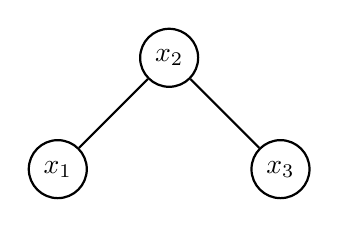
\begin{tikzpicture}[thick, node distance = {20mm}, main/.style = {draw, circle}] 
			\node[main] (1) {$x_1$}; 
			\node[main] (2) [above right of=1] {$x_2$};
			\node[main] (3) [below right of=2] {$x_3$};
			
			\draw (1) -- (2);
			\draw (2) -- (3);
		\end{tikzpicture}
		\caption{Basic Graph}
		\label{basic-graph}
	\end{subfigure}
	\hfill
	\begin{subfigure}{.32\textwidth}
		\centering
		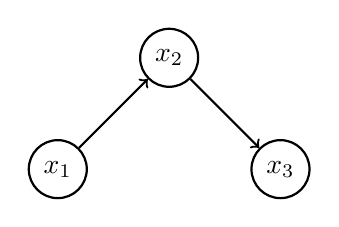
\begin{tikzpicture}[thick, node distance = {20mm}, main/.style = {draw, circle}] 
			\node[main] (1) {$x_1$}; 
			\node[main] (2) [above right of=1] {$x_2$};
			\node[main] (3) [below right of=2] {$x_3$};
			
			\draw[->] (1) -- (2);
			\draw[->] (2) -- (3);
		\end{tikzpicture}
		\caption{Directed Graph}
		\label{directed-graph}
	\end{subfigure}
	\hfill
	\begin{subfigure}{.32\textwidth}
		\centering
		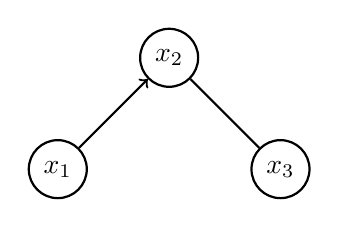
\begin{tikzpicture}[thick, node distance = {20mm}, main/.style = {draw, circle}] 
			\node[main] (1) {$x_1$}; 
			\node[main] (2) [above right of=1] {$x_2$};
			\node[main] (3) [below right of=2] {$x_3$};
			
			\draw[->] (1) -- (2);
			\draw (2) -- (3);
		\end{tikzpicture}
		\caption{Mixed Graph}
		\label{mixed-graph}
	\end{subfigure}

	\caption{Example of (\textbf{a}) a simple graph, (\textbf{b}) a directed graph, and (\textbf{c}) a mixed graph.}  
\end{figure}

A graph is called \emph{bi-partite} if it possible to separate the set of vertices in two separate sets, such there exists only edges between vertices that are in the two separate sets. The structure of the graph can be used to analyze how things relate to each other. 
Consider the situation of geographical maps, we can model countries as vertices and create an edge between two countries if they are neighboring. Then, we can use the graph structure to analyze how many possible paths there are from one country to another where only a maximum of two other countries are crossed. For many use cases, however, it is useful to let graph contain data or have less restrictive rules on how a graph might be formed.

\paragraph{Directed Edges} The most basic extension of graphs is that they are allowed directed edges. This means that there exists an edges from one node to another, but that this connection does not exists in the opposite direction. In the case of countries and their neighbors, this does not make sense; if one country borders another, the opposite is true as well. However in the case of the internet, one website might contain a hyperlink to another, while the opposite does not have to be the case. We need directed graphs to properly model the situation. Again, we can use this model to see how many paths there are from one website to another, with the restriction of visiting 2 other websites in between. In this case the $E$ is a set of ordered pairs of vertexes:
\begin{equation}
	E = \left\{\left(v_1, v_2\right) | \left(v_1, v_2\right) \in V^2\text{ and } v_1 \neq v_2 \right\}
	\label{directed-edges}
\end{equation}
\Cref{directed-graph} shows an illustration of the following directed graph:
$V = \left\{x_1, x_2, x_3\right\}$ and $E = \left\{\left(x_1, x_2\right), \left(x_2, x_3\right)\right\}$

\paragraph{Mixed Graphs}
Mixed graphs are graphs that accepted both undirected and directed edges. In that case a graph is defined with two sets of edges; where one set describes the undirected edges and the other the directed edges:
\begin{equation}
	G = \left\{V, E_1, E_2\right\}
\end{equation}
with $E_1$ and $E_2$ being defined as edges as presented in \cref{undirected-edges,directed-edges} respectively. \cref{mixed-graph} shows the illustration of a mixed graph:
$V = \left\{x_1, x_2, x_3\right\}$, $E_1 = \left\{\left\{x_1, x_2\right\}\right\}$, and $E_2 = \left\{\left(x_2, x_3\right)\right\}$.
Mixed graphs are sometimes used in applications where the direction of an edge is unclear, but where you know a relation exists. Types of these graphs appear, for example, in causality research. 

\subsection{Graphs + Data}
The types of graphs we described are all graphs that do not contain data themselves, we can only reason about the structure of the graphs themselves. 

\section{Reproducible Science}
In order to establish experimental results in science, it is essential that results can be independently verified. Many different fields have had problems where the reproducibly of scientific studies was lacking. In field of psychology, a large reproducibility study was carried out~\citep{psychology-reproduciblity}. In this study a selection of 100 published studies in 2008 were taken, the goal was to reproduce the findings of all these studies to determine how many were holding up. Of the original 100 studies, 97 presented significant results. When trying to reproduce these results, for only 35 out of 97 these studies, it was possible to reproduce significant results. 

It is not entirely clear why this many scientific studies were not reproducible. But, it seems many type II errors happened; failing to reject the null-hypothesis while it is false. Scientific misconduct could explain some of these results, but it is unlikely that this is happening at such a large scale. All studies that this project tried to reproduce were published in a just three journals. These journals were peer reviewed; only the scientific studies the reviewers thought were good enough are published. This process of course introduces a selection bias, studies that show more impactful results have a higher probability of being published. This bias favors papers in which type II errors are being made, even though the scientific conduct was proper. 

When a scientific study is published, people might interpret its results as fact. Something that should not be done of course, one should consider a scientific results only as evidence for how the world might work. Then, every time the results are reproduced, more evidence is gather to support the findings. By reproducing science, our understanding of the words becomes clearer, and eventually we can assume with a high certainty that something is true. 

In the field of information retrieval, reproducibility has also been a topic of interest. Throughout this thesis the topic of reproducibility will come back, here I will only highlight some observations on the topic of reproducibility in our field, and some closely related issues. Before introducing these observations it is important to clearly define what is meant by reproducibility. Within ACM there has been made a clear distinction between the concepts of; repeatability, replicability, and reproducibility. 
\begin{itemize}
	\item \emph{Repeatability} is verification of results produced by the \underline{same} research group, using the \underline{same} resources. Basically, confirming that when you run your own code, the systems produces the same results consistently. This might seem trivial, but it might happen that when you update software to some newer version, e.g.\ upgrading from Lucene 7 to Lucene 8, the results your software produces might slightly differ. 
	\item \emph{Replicability} is the verification of results produced by a \underline{different} research group, but using the \underline{same} resources. This could, for example, be done by running the publicly available code for a research project and verifying its results. This is already somewhat more tricky than it might look. Often, in scientific papers, parameters settings of the software might be left out, making it hard to correctly verify results. 
	\item \emph{Reproducibility} is the verification of results produced by a \underline{different} research group that uses its own (\underline{different}) resources. Typically, in a reproduction study the scientific study is done from scratch using the instruction as presented in a paper. As many details might be left out, its even harder to reproduce results exactly. However, if a reproduction study is able to confirm the results of previous work, this is a strong indication that the results presented in that work are correct.
\end{itemize}

In \cref{ir-using-relational-databases}, we will present some scientific results about the BM25 algorithm. But basically, many systems implement this algorithm, while the reported effectiveness results as measured through established metrics (a subset of metrics described in \cref{sec:evaluation}) are quite different. How this can happen will be discussed. BM25 however is a ranking method that is often used as a baseline method. When comparing newer algorithms to BM25, it makes quite a difference if its implementation reports a low score to a relatively high score. 

\Citet{Armstrong-dontaddup} showed that many improvements of ranking algorithms presented throughout the years, did not add up. In many cases where significant improvements were presented, they were compared against weak baselines. Also, there was no upward trend of retrieval effectiveness, which would be expected if we find improvement over and over again. More recently, \citet{weak-baselines} showed that this is still happening, new methods are being compared against implementations of BM25 that have non optimal hyper parameter settings. This leads to methods looking better than they actually are, and it is harder to compare methods against each other if the baseline that was compared against is not identical.

For this thesis, all software and data produced is publicly available and released on Zenodo\footnote{\url{https://zenodo.org}, last accessed - May 16th 2023} in order to facilitate reproducible science, following the guidelines of the research data management policy of the Institute for Computing and Information Science of the Radboud University\footnote{\url{https://www.ru.nl/icis/research-data-management/}}. Additionally, in some chapters the importance of reproducibility will be highlighted and be discussed in more detail.  
\chapter{IR using Relational Databases}
\section{Introduction}
Where commonly information retrieval researchers use inverted indexes as data structures, there is also a rich history of researchers using relational databases for representing the data in information retrieval systems. 

% Describe boolean retrieval systems
% Describe other systems by for example Norbert 

In a more recent work \cite{OldDog} showed that the common used BM25 ranking function can also be easily expressed using relational tables. Their work specifically focused on the retrieval efficiency of several systems.   
% End with OldDog system by Hannes

\section{Reproducibility}

We \cite{Kamphuis2020BM25}
\chapter{From Tables to Graphs}
\label{from-tables-to-graphs}
\epigraph{``The reader will have anticipated that I have no very convincing
	arguments of a positive nature to support my views. If I had I should not
	have taken such pains to point out the fallacies in contrary views.``}{Alan Turing - 1950}

\begin{Abstract}
	\begin{changemargin}{1cm}{1cm}
		This chapter introduces GeeseDB. GeeseDB is a Python toolkit for solving information retrieval research problems, that leverages graphs as data structures. It aims to simplify information retrieval research by allowing researchers to formulate graph queries through a graph query language. GeeseDB is built on top of DuckDB, an embedded column-store relational database for analytical workloads. GeeseDB is available as an easy-to-install Python package. In only a few lines of code, users can create a first-stage retrieval ranking using BM25. Queries read and write Numpy arrays and Pandas dataframes at negligible data transformation cost. Therefore, the results of a first-stage ranker expressed in GeeseDB can be used in various stages in the ranking process, enabling all the power of Python machine learning libraries with minimal overhead.
	\end{changemargin}
\end{Abstract}

\section{Introduction}
In recent years there has been a lot of exciting new information retrieval research that uses non-text data to improve the efficacy of search applications. All these research directions have improved search systems' effectiveness by using more diverse data. Although more diverse data sources are considered, these systems are often implemented through a coupled architecture. In particular, first-stage retrieval is often carried out with different software than that used in later retrieval stages, where these novel reranking techniques tend to be used. In our view, researchers could benefit from a system where retrieval stages are more tightly coupled, which facilitates the exploration of how to use non-content data for ranking and serves the data in a format suitable for reranking with, e.g., transformers, tree-based methods or graph-based methods.

The previous chapter demonstrates how relational databases can be used for information retrieval problems. Integrating alternative data sources into search systems is easier when using a relational database instead of an inverted index. In the case of information retrieval, graph data can often be used to improve search effectiveness. One of the most famous examples where graphs help information retrieval is the PageRank algorithm~\citep{pagerank}. Although it might be possible to express ranking over graph data in relational databases, they are not designed with graph structures in mind. 

The data management community has shown much interest in graph databases in recent years. Graph databases are different from relational databases in that graphs are the main representation for managing the data, instead of the usual relations. Graphs can be considered a better abstraction for real-world data than relations. Graphs focus much more on concepts (nodes in a graph) and how they relate to each other (edges in a graph), while in a relational database this information is implicit, requiring knowledge of the schema. From the types of graphs discussed in \cref{related-work}, we focus on using \emph{property graphs} in this chapter. This type of graph contains nodes and directed edges, which can be labeled; nodes and edges can also have associated key-value pairs.

The research goal in this chapter is two-fold; firstly, we develop a system that can search efficiently in information represented as graphs. In the previous chapter, we showed that relational databases could search efficiently and help reproducible research. However, these systems do not support graph data structures directly in their interface to the user (e.g., the query language). Systems built on inverted indexes use coupled architectures, which can introduce unnecessary overhead.

Secondly, we want to create a system where both first and second-stage retrieval are directly supported. In IR research, multi-stage retrieval systems contain components that are not run in the same ecosystem; introducing overhead in retrieval efficiency. 
So in this chapter, the prototype system GeeseDB is introduced; it tries to leverage the same techniques for search as relational databases do while also naturally being able to support graphs. This leads to the main research question for this chapter:

\begin{itemize}
	\item[\textbf{RQ2:}] Can we extend the benefits from using relational databases for information retrieval to using graph-databases while being able to express graph-related problems easier?
\end{itemize} 

In order to answer this research question, we will use our own prototype system GeeseDB. Before introducing GeeseDB, we first look into work that uses systems that combine two systems for two-stage retrieval experiments, and systems built for processing graphs.

% rewrite and reflect on the previous chapter, and give context in which graph databases are helpful.

\section{Related work }
% Describe the related work which was presented in the GeeseDB paper, but also include more related work regarding approaches that use graph language-like approaches (different subsection). 
In modern IR it is not uncommon to use coupled architectures. In many situations a ranking model is used that is efficient, but only reasonably effective. BM25 can be considered a model that can be calculated cheaply providing a good score for a more advanced (but less efficient) retrieval model that could achieve higher effectiveness. In such cases, BM25 can be used to calculate an initial top-$k$ ranking that contains (presumably) all relevant documents. Then, the more expensive model only has to calculate the final ranking scores over the top-$k$ documents.

In this section we start discussing methods that implement multi-stage approaches, then systems that implement them are highlighted. In particular there will be a focus on the coupled-architectures aspect of these systems. Finally, some proposed methods will be discussed to deal with cons arising from coupled architectures. 

\subsection{Learning To Rank}
In learning-to-rank (LTR), multi-stage retrieval approaches are widely used; LTR models are not efficient enough to compute a relevance score value for all documents in the collection.
In these cases, a decision tree based ensemble like LambdaMART~\citep{lambdamart} tends to be trained. These models take input that is usually not stored in an inverted index. So, in order to use these models, the output from the inverted index needs to be combined with other data.

\Citet{ltr-1} showed that for the TREC Contextual Suggestion track~\citep{contextual-suggestion-track}, reranking using user-based features significantly improved retrieval effectiveness over a baseline language modeling approach. These features show that data not present in the document's text can help the retrieval effectiveness of systems; metadata helps to rank. 

\Citet{ltr-2} show examples of features that have been effective for learning to rank, many of these features are non-textual. Some influential features are: click count, click entropy, and the number of displayed results in a session. 

\subsection{Dense Retrieval}
Where traditionally, search was carried out using inverted indexes, neural retrieval has become more prevalent in recent years. When neural retrieval \citep{neural-ir} is implemented as a vector search approach, it is referred to as dense retrieval.
Consider, for example, the work by \citet{dense-retrieval-1}; in their work, they proposed \texttt{clear}, a model that aims to complement lexical models with a dense retrieval model. In their study, they use BM25 as the lexical model. The BM25 scores are calculated using an inverted index (Anserini~\citep{anserini}), while the dense retrieval model is a fine-tuned BERT bi-encoder. This dense model calculates a score using a different maximum inner-product search (MIPS) system (Faiss~\citep{faiss}) to calculate a similarity score for the query document pairs. Then scores are weighted and summed to calculate a new ranking score value. 

In a similar study, \citet{dense-retrieval-2} compared several methods on the MS Marco document and passage datasets. In their work, one of the two best models on the passage dataset was to combine a lexical model with a BERT-based bi-encoder. The scores were combined by retrieving the top-\textit{n} documents for both the lexical model and the bi-encoder. In order to do this, an inverted index (Anserini) is used to retrieve the documents for the lexical model, while the bi-encoder uses a MIPS system (ScaNN~\citep{scann}).

A third example, is the study of  \citet{dense-retrieval-3} that experiments with distilled dense representations. They do an extensive comparison study, and in their work, the best results are reported by either multi-stage or hybrid dense + sparse retrieval methods. The multi-stage retrieval method used BM25 in combination with BERT-large. Although effective, it is a method with a high latency because of the cross-encoder used. A TCT-ColBERT (Tightly-Coupled Teacher - ColBERT) bi-encoder with doc2query-T5 sparse retrieval was the best hybrid method. This sparse retrieval method is a BM25 retrieval method that expands the documents with T5 language model questions~\citep{2020t5}. These questions were generated by letting the T5 language model generate questions that the passage might answer. Sparse retrieval is carried out by Anserini, and dense retrieval by Faiss. 

\subsection{Knowledge Graphs and Entities}
% knowledge graphs to leverage entity information~\cite{entity-1, entity-2, entity-3}, 
Knowledge graphs have been used a lot as well in IR research. \Citet{entity-1} proposed the Entity Linking incorporated Retrieval (ELR) approach. The idea behind this concept is that when entity annotations are available for queries and documents, they can be incorporated into the ranking model. Their publication only focuses on entity retrieval, but the method can generalize to ad-hoc document and passage retrieval. The entities are incorporated by creating a dedicated index for entities on which entity scores can be calculated. These are then merged by the document scores calculated using the regular index. By incorporating entity scores, ELR has been shown to increase effectiveness scores for multiple baseline methods. 

\Citet{entity-3} also used entity features for query expansion. One of the features was calculated by tagging queries with an entity-linking system. When entities were found, information from the knowledge base linked to them was included in query expansion. Alternative names of the entity were also included in the query expansion. Then, this expanded query provided a score for all documents. Another feature they calculate is obtained by ranking the entities in the knowledge base using the original query text. Then the data (e.g., words in the descriptions) included in the knowledge base can be included as terms for query expansion. Multiple other features using entities were also calculated, 

For additional background related to entities in search, refer to \Citet{entity-2}, an excellent book on entity-oriented search, that surveys many methods that use entities for search. 

Basically, in order to include entities, a knowledge graph needs to be queried. This tends to be done by a different systems than the systems used for regular retrieval. If we could integrate IR in graph databases, a single system would solve the complete process.
% maybe include a subsection about graphs including the work by mcdonald

\subsection{Current approaches}
Recently, retrieval methods using neural networks have become state-of-the-art, mainly using large language models. In this section the two most commonly used research systems are described, highlighting how they with neural approaches to IR.
PyTerrier~\citep{pyterrier} and Pyserini~\citep{pyserini} are modern research systems that are widely used for information retrieval research. These systems are built as inverted index systems, with a separate component to handle neural retrieval models. 

\subsubsection{PyTerrier}
PyTerrier by~\citet{pyterrier}, is a Python extension of Terrier~\citep{terrier}. Terrier is an open-source search engine system written in Java. It implements state-of-the-art indexing and retrieval techniques on top of an inverted index. It is a system suited for rapidly developing retrieval experiments concerning document collections with many documents. 
The PyTerrier extension was developed to express complex IR pipelines in Python. Using Python operators directly, it is possible to set up an IR pipeline using PyTerrier in only a few lines of code. 

PyTerrier was expanded to support state-of-the-art large language model reranking approaches and dense retrieval methods. As the PyTerrier framework is developed for the Python ecosystem, other (re-)ranking methods that are implemented in Python can readily work with PyTerrier. The PyTerrier system is ideal for modern information retrieval research, that often concerns reranking through learned methods, as they are often developed in Python.

Note, however, that PyTerrier uses a coupled architecture. First-stage retrieval is carried out using Terrier in Java (e.g., a BM25 run), and then the resulting top documents are reranked in Python. For this, some overhead is introduced because of data transfer between processes. 

\subsubsection{Pyserini}
Pyserini was developed by~\citet{pyserini}, which is a Python extension of Anserini~\citep{anserini}. Pyserini and Anserini have a lot in common with PyTerrier and Terrier. Just like Terrier, Anserini is developed in Java, but on top of Apache Lucene. Anserini is developed as a system with solid support for reproducible research. Anserini provides reproducible baselines for many retrieval benchmarks that can be run with minimal investment of resources. 

Pyserini is developed as a Python wrapper around the Anserini retrieval system. Within the Python ecosystem, it is possible to access the Anserini internals and replicate the same experiments implemented in Anserini. Similarly to PyTerrier, Pyserini also contains features that are not available directly in Anserini; ranking methods that make use of large language models, such as dense retrievers and BERT-based cross encoders. As these methods are generally developed in Python, it is much easier to support them with Pyserini compared to Anserini.

Anserini is included in Pyserini as a JAR file, so when using Pyserini for first-stage retrieval, data needs to be retrieved from JAVA before it can be materialized in Python. The setup is similar to that of Pyterrier. 

\subsection{Proposed approaches}
% Paper van Jimmy op DESIRES is belangrijk. 
\subsubsection{Separation of the Logical and Physical Model}
% todo different compontent systems?? ask Arjen what it says?
As shown in the previous sections, dense and sparse retrieval methods are often implemented using different  systems, which  introduces the coupled architecture. \citet{seperation-logical-physical} recognizes that sparse retrieval models tend to be implemented using inverted indexes and dense retrieval methods with approximate nearest neighbor systems. Although these systems are different, the input and the output are the same: the input is a query, and the output is a ranked list of the top-$k$ documents the ranking methods deem the most relevant. 

In order to be able to formalize these similarities and distinctions more clearly, \citeauthor{seperation-logical-physical} proposes a distinction between the logical and physical retrieval models. Logical models specify encoders that map documents and queries to a representation, and a comparison function that defines how a ranking score value can be computed from comparing these representations. Physical models define how to create a top-$k$ ranking from a large corpus given a query. The most straightforward physical approach would simply apply the logical model to every query-document pair, but through optimizations it might not necessary to compare all documents to the query. For example, dense retrieval methods often make use of the HNSW datastructure for nearest neighbor search~\citep{faiss} which prunes documents that have a low likelihood of being relevant. 

\subsubsection{A Graph Query Language for IR}
% Reproducible IR needs a graph query language ook belangrijk
It would be ideal for a system to encapture these different ways of approaching IR research natively; work with multiple stages in the ranking process, but also reason about entities and knowledge graphs. 
\citet{need-graph-db} proposed to use a graph query language for information retrieval problems. In the context of separating logical and physical models, a graph query language can be interpreted as a logical model, while the engine that implements the graph query language can be considered the physical model.

If it is possible to express both first stage and second stage retrieval in such a query language, both stages would be computed by the same physical model, automatically ensuring a coupled architecture is not necessary. Having a graph query language available, ensures that more complicated retrieval strategies can be expressed compared to when a relational query language is used. 

So ideally we develop a system with the following two capabilities; the system supports first retrieval stage directly, and graph queries over the output of this first stage retrieval can be processed without a coupled architecture. In order to fulfill these needs, we developed GeeseDB in a follow up study. 

\section{GeeseDB}
% Introduce GeeseDB, and the approach of what we are doing with GeeseDB
GeeseDB\footnote{\url{https://github.com/informagi/geesedb}, last accessed January 22th 2024} is a prototype Python toolkit for information retrieval that leverages graphs as data structures, allowing metadata and graph-oriented data to be easily included in the ranking pipeline. The toolkit is designed to quickly set up first-stage retrieval and make it easy for researchers to explore new ranking models. 

In short, GeeseDB aims to provide the following functionalities:
\begin{itemize}
	\item GeeseDB is an easy-to-install, self-contained Python package available through \texttt{PyPI} with as few as possible dependencies. It contains topics and relevance judgments for several standard IR collections out-of-the-box, allowing researchers to develop new ranking models quickly. 
	\item First stage (sparse) retrieval is directly supported. In only a few lines of code, it is possible to load documents and create BM25 rankings. 
	\item Data is served in a usable format for later retrieval stages. GeeseDB allows directly running queries on Pandas data frames for efficient data transfer to sequential reranking algorithms.
	\item Easy data exploration is supported through querying data with SQL, but more interestingly, using a graph query language (based on the Cypher query language), making exploring new research avenues easier. This prototype supports a subset of the graph query language Cypher, similar to the property graph database model query language as described by~\citet{angles2018property}.
\end{itemize}

\section{Design}
% Expand the Design part a lot, how did we solve certain technical problems. 
At the core of GeeseDB lies the full-text search design presented by~\citet{OldDog} as discussed already in~\cref{ir-using-relational-databases}. This work proposes a column-store database for IR prototyping, which uses the database schema described in~\cref{olddog_schema}, consisting of three database tables.
\begin{figure}
	\centering
	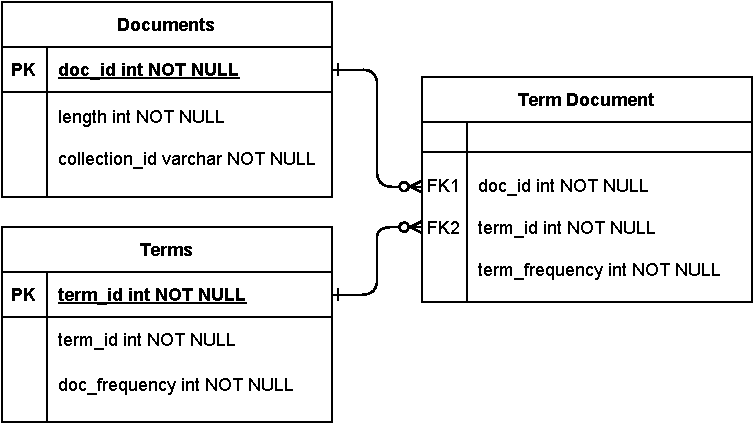
\includegraphics[width=\linewidth]{./imgs/olddog-schema-2.pdf}
	\caption{Database schema by \citeauthor{OldDog} for full text search in relational databases}
	\label{olddog_schema}
\end{figure}
Using these three tables, the authors show that BM25 can be easily expressed as a SQL query with latencies on par with custom-built IR engines. In GeeseDB, we use the same relational schema for full-text search.
Instead of seeing the document data and term data as tables that relate to each other through a many-to-many join table, it is also possible to consider this schema as a bipartite graph. In this graph, documents and terms are considered nodes connected through edges. If a term occurs in a document, an edge exists between that term and the document. GeeseDB uses the data model of property graphs labeled multigraphs where both edges and nodes can have property-value pairs. The database schema, as described in~\cref{olddog_schema}, would then translate to the property graph schema shown in~\cref{olddog-graph-schema}.
\begin{figure}
	\centering
	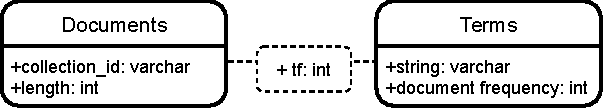
\includegraphics[width=\linewidth]{./imgs/olddog-graph-schema.pdf}
	\caption{Graph schema representing bipartite document-term graph}
	\label{olddog-graph-schema}
\end{figure}
A small example of a graph represented by this schema is shown in~\cref{example-olddog-graph}. Document nodes contain document-specific information (i.e., document length and the collection identifier), term nodes contain information relevant to the term (i.e., the term string and the term's document frequency), and the edges between document and term nodes contain term frequency information (i.e., how often is the term mentioned in the document represented the respective nodes it connects).
%\begin{figure}
%	\centering
%	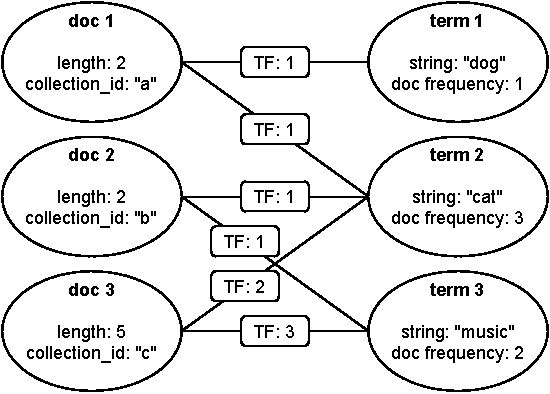
\includegraphics[width=\linewidth]{./imgs/example_olddog_graph.pdf}
%	\caption{Example term-document graph that maps to relational database schema}
%	\label{example-olddog-graph}
%\end{figure}

\begin{figure}
	\centering
	\begin{tikzpicture}[thick, node distance = {60mm}, main/.style = {draw, ellipse}] 
		\node[main, align=center, shape=ellipse] (1) {\underline{doc 1} \\ \textit{collection id:} "a" \\ \textit{len:} 2}; 
		\node[main, align=center] (2) [right of=1] {\underline{term 1} 
		\\ \textit{doc frequency:} 1 \\ \textit{string:} "dog"};
		
		\node[main, align=center, shape=ellipse, node distance=25mm] (3) [below of=1] {\underline{doc 2} \\ \textit{collection id:} "b" \\ \textit{len:} 2}; 
		\node[main, align=center, node distance=25mm] (4) [below of=2] {\underline{term 2} \\ \textit{doc frequency:} 2 \\ \textit{string:} "cat"};
		
		\node[main, align=center, shape=ellipse, node distance=25mm] (5) [below of=3] {\underline{doc 3} \\ \textit{collection id:} "c" \\ \textit{len:} 2}; 
		\node[main, align=center, node distance=25mm] (6) [below of=4] {\underline{term 3} \\ \textit{doc frequency:} 5 \\ \textit{string:} "music"};
		
		\draw (1) edge[align=center, bend left=10] node[above] {\textit{TF:} 1} (2);
		\draw (1) edge[align=center] node[yshift=1mm, above] {\textit{TF:} 1} (4);
		\draw (3) edge[align=center, bend left=10] node[above] {\textit{TF:} 1} (4);
		\draw (3) edge[align=center, bend left=20] node[yshift=-1mm, left] {\textit{TF:} 1} (6);
		\draw (5) edge[align=center, bend right=20] node[yshift=1mm, left] {\textit{TF:} 2} (4);
		\draw (5) edge[align=center, bend right=10] node[below] {\textit{TF:} 3} (6);
		
		
	\end{tikzpicture}
	\caption{Example term-document graph that maps to relational database schema}
	\label{example-olddog-graph}
\end{figure}

If one wants to, for example, also store position data, this graph can easily be extended to a graph where the edges store term positions. If a term appears multiple times in a document, the property graph model will allow multiple edges between two nodes. The graph schema that we described by~\cref{olddog-graph-schema} maps one-to-one to the relational database schema described by~\cref{olddog_schema}, when we represent nodes by standard relational tables that represent specific data units (terms, documents), while many-to-many join tables represent the edges. So, even though we think of the data as graphs, they are still represented as relational tables in the backend. When using GeeseDB for search, we at least expect the document-term graph to be present. New node types can be introduced to explore new search strategies. 

\subsubsection{Backend}
GeeseDB is built on top of DuckDB~\citep{duckdb}, an in-process SQL OLAP (analytics optimized) database management system. DuckDB is designed to support analytical query workloads. It aims explicitly to process complex, long-running queries where a significant portion of the data is accessed, conditions matching the case of IR research. DuckDB has a client Python API which can be installed using \texttt{pip}\footnote{\url{https://duckdb.org/docs/installation/?version=stable&environment=python}, last accessed March 2nd 2024}. Afterward, it can be used directly. DuckDB has a separate API built around NumPy\footnote{\url{https://numpy.org/}, last accessed March 2nd 2024} and Pandas\footnote{\url{https://pandas.pydata.org/}, last accessed March 2nd 2024}, providing NumPy/Pandas views over the same underlying data representation without incurring data transfer (usually referred to as ``zero-copy'' reading). Pandas DataFrames can be registered as virtual tables, allowing to query the data in Pandas DataFrames directly. GeeseDB inherits all these functionalities from DuckDB.

As DuckDB is a database management system, we can execute analytical SQL queries on tables containing our data, including the BM25 rankings described by~\citet{OldDog}. By default, the BM25 implementation provided with GeeseDB implements the disjunctive variant of BM25 instead of the conjunctive variant they used. Although the conjunctive variant of BM25 can be calculated more quickly, the differences between effectiveness scores are noticeable on smaller collections. Also, disjunctive would mostly likely better match the mental model of our IR researchers as GeeseDB users. For now, we only support the original formulation of BM25 by~\citet{bm25-robertson}. However, supporting other versions of BM25 as described in the previous chapter is trivial.

\section{Graph Query Language}
GeeseDB distinguishes itself from alternatives, database-backed (OldDog)~\citep{olddog-docker}, or native systems (Anserini~\citep{anserini}, Terrier~\citep{terrier}) by offering a graph query language, based on Cypher~\citep{cypher}. 
For now, GeeseDB implements Cypher's basic graph pattern-matching queries for retrieving data. An example of a graph query supported by GeeseDB is presented in~\cref{fig:graph_query}.
\begin{figure}
	\begin{minted}[linenos]{cypher}
MATCH (d:docs)-[]-(:authors)-[]-(d2:docs)
WHERE d.collection_id = "96ab542e"
RETURN DISTINCT d2.collection_id
	\end{minted}
	\caption{An example cypher query that finds all documents that were written by the same author that wrote the document with the \texttt{collecion\_id} ``96ab542e''}
	\label{fig:graph_query}
\end{figure}
This co-authorship query finds all documents written by the same authors as those who wrote document ``96ab542e''. For comparison, ~\cref{fig:corresponding_sql} illustrates the same query represented in SQL; much more complex than the Cypher version, due to the join conditions that have to be made explicit. In order to connect the ``docs''-table with the ``authors''-table two joins are needed; reconnecting the ``docs'' table again introduces two more joins.

\begin{figure}
	\begin{minted}[linenos]{sql}
SELECT DISTINCT d2.collection_id
FROM docs AS d2
JOIN doc_author AS da2 ON (d2.collection_id = da2.doc)
JOIN authors AS a2 ON (da2.author = a2.author)
JOIN doc_author AS da3 ON (a2.author = da3.author)
JOIN docs AS d ON (d.collection_id = da3.doc)
WHERE d.collection_id = '96ab542e'
	\end{minted}
	\caption{SQL query that corresponds to the graph query described in Figure~\ref{fig:graph_query}.}
	\label{fig:corresponding_sql}
\end{figure}

The current implementation of  GeeseDB supports the following Cypher keywords: \texttt{MATCH}, \texttt{RETURN}, \texttt{WHERE}, \texttt{AND}, \texttt{DISTINCT}, \texttt{ORDER BY}, \texttt{SKIP}, and \texttt{LIMIT}. Instead of using \texttt{WHERE} to filter data, it is also possible to use graph matching patterns that include filters; as shown in~\cref{fig:graph_query2}; the query returns the length of document ``96ab542e''. Here the filter is defined between the curly braces. 
\begin{figure}
	\begin{minted}[linenos]{cypher}
MATCH (d:docs {d.collection_id: "96ab542e"})
RETURN d.len
	\end{minted}
	\caption{Graph query where the length of document with \texttt{collection\_id} is returned.}
	\label{fig:graph_query2}
\end{figure}
Everything that is not directly supported yet by our implementation can, of course, still be expressed in SQL, which is fully supported. \footnote{GeeseDB supports the graph queries by translating them to their corresponding SQL queries. After all, both nodes and edges are just tables in the backend.} In order to know how to join nodes to each other if no edge information has been provided, GeeseDB stores information on the graph schema. This way, GeeseDB knows how nodes relate to each other through which edges. 

\section{Usage}
GeeseDB comes as an easy-to-install Python package that can be installed using pip, the standard package installer for Python:

\begin{verbatim}
	$ pip install geesedb
\end{verbatim}
After installing GeeseDB, we can immediately start using it. It is also possible to install the latest commit by installing the latest version directly from GitHub.
As an example, we will show how to use GeeseDB for the background linking task of the TREC News Track~\citep{soboroff2018trec}. The goal of this task is: \textit{Given a news story, find other news articles that can provide meaningful context or background information.} These articles can then be recommended to the reader to help them understand the context in which these news articles occur. The collection used for this task is the Washington Post V3 collection\footnote{\url{https://trec.nist.gov/data/wapost/}, last accessed March 2nd 2024} released for the 2020 edition of TREC. It contains $671,945$ news articles published by the Washington Post between 2012 and 2020, and 50 topics with relevance assessments (topics correspond to collection identifiers of documents for which relevant data has to be found). The articles in this collection contain valuable metadata; in particular, we will investigate how to best use the article authorship information. We extracted $25,703$ unique article authors, where it is possible that multiple authors co-wrote a news article. We also annotate documents with entity information which was obtained by using the Radboud Entity Linker~\citep{rel}. In total $31,622,419$ references to $541,729$ unique entities were found. The links also contain mention and location information, as well as the entity type (\texttt{ner\_tag}) found by the linker's entity recognition module (The entity type is part of a link, as the entity linker can assign different tags to the same entity.) \Cref{fig:geesedb-graph} illustrates the data schema that we use for the background linking task. 

\begin{figure}
	\centering
	\begin{tikzpicture}[thick, node distance = {40mm}, main/.style = {draw, rectangle}] 
		\node[main, align=center, shape=ellipse] (1) {\underline{Documents} \\ \textit{len:} 3  \\ \textit{collection\_id:} "abc"}; 
		\node[main, align=center] (2) [above right of=1] {\underline{Authors} \\ \textit{Name:} "Arjen"};
		\node[main, align=center, shape=ellipse] (3) [below right of=2] {\underline{Documents} \\ \textit{len:} 2 \\ \textit{collection\_id:} "def"};
		\node[main, align=center] (4) [above right of=3] {\underline{Authors} \\ \textit{Chris:} "Chris"};
		
		\node[main, align=center, shape=rectangle] (5) [below of=1] {\underline{Terms} \\ \textit{string:} "dog" \\ \textit{df:} 1};
		\node[main, align=center, shape=rectangle] (6) [right of=5] {\underline{Terms} \\ \textit{string:} "cat" \\ \textit{df:} 2};
		\node[main, align=center, shape=rectangle] (7) [right of=6] {\underline{Terms} \\ \textit{string:} "music" \\ \textit{df:} 1};
		
		\node[main, align=center, shape=ellipse] (8) [above right of=2] {\underline{Entities} \\ \textit{entity:} "dog" \\ \textit{df:} 1};
		
		
		\draw (1) -- (2);
		\draw (2) -- (3);
		\draw (3) -- (4);
		
		\draw (5) edge[align=center] node[left] {\textit{tf:} 1} (1);
		\draw (6) edge[align=center, bend left=10] node[right] {\ \textit{tf:} 2} (1);
		\draw (6) edge[align=center] node[left] {\textit{tf:} 1} (3);
		\draw (7) edge[align=center] node[left] {\textit{tf:} 1} (3);
		
		\draw (1) edge[align=center, bend left=45] node[above, left] 
		{\textit{mention:} "dog"\\\textit{ner\_tag:} "misc"\\\textit{start:} 0\\\textit{len:} 1} (8);
	\end{tikzpicture}
	\caption{Example property graph for the TREC News Track's background linking task. The node types are authors, entities, terms, and documents. Edges connect document nodes to other types of nodes. Both edges and nodes can have properties (following the property graph model). Multiple edges may exist between one entity node and one document node, as one entity can be linked multiple times to one document.}
	\label{fig:geesedb-graph}
\end{figure}

\subsection{Indexing and Search}
In order to start, a database containing at least the document and term information needs to be created. Figure \ref{fig:load_text_data} shows how the data can be easily loaded using CSV files.
\begin{figure}
	\begin{minted}[linenos]{python}
from geesedb.index import FullTextFromCSV

index = FullTextFromCSV(
    database='/path/to/database',
    docs_file='/path/to/docs.csv',
    term_dict_file='/path/to/term_dict.csv',
    term_doc_file='/path/to/term_doc.csv'
)
index.load_data()
	\end{minted}
	\caption{Load text data from the WashingtonPost collection formatted as CSV files in the format as described by~\citet{OldDog}}
	\label{fig:load_text_data}
\end{figure}

Instead of loading the data from CSV files, it is also possible to load the text data directly using the CIFF format for information retrieval data exchange~\citep{ciff}. GeeseDB also has functionalities to create CSV files from the CIFF format. Authorship information and entity links are loaded similarly. After loading the data, we can easily create a BM25 ranking for ad hoc search in the Washington Post collection, as shown in~\cref{fig:code_bm25_ranking}.

\begin{figure}
	\begin{minted}[linenos]{python}
from geesedb.search import Searcher

searcher = Searcher(
    database='/path/to/database', 
    n=10
)
hits = searcher.search_topic('obama and trump')
	\end{minted}
	\caption{Example on how to create a BM25 ranking for the query ``obama and trump'' that returns the top 10 documents.}
	\label{fig:code_bm25_ranking}
\end{figure}

For the background linking task, however, we do not have regular topics; we only have the document identifiers of the documents for which we need to find relevant background info. In order to search for relevant background reading, queries that represent our information need have to be constructed. A common approach uses the top-$k$ TF-IDF terms of the source article~\citep{anserini-news}. These can easily be found using the Cypher statement in~\cref{fig:tfidf-cypher}. Instead of using Cypher, it would also be possible to use SQL, as shown in~\cref{fig:tfidf}; however, this example shows again that the Cypher query is more elegant than SQL, and easier to comprehend. 

\begin{figure}
	\begin{minted}[linenos, escapeinside=||]{cypher}
MATCH (d:docs {collection_id: |?|})-[]-(t:term_dict)
RETURN string
ORDER BY tf*log(671945|/|df)
DESC
LIMIT 5
	\end{minted}
	\caption{Prepared\footnote{Prepared means that parameters are provided at query time. In this case the question mark.} Cypher statement that finds the top-$5$ TF-IDF terms in a given document.}
	\label{fig:tfidf-cypher}
\end{figure}
\begin{figure}
	\begin{minted}[linenos]{sql}
SELECT term_dict.string
FROM term_dict
JOIN term_doc ON (term_dict.term_id = term_doc.term_id)
JOIN docs ON (docs.doc_id = term_doc.doc_id)
WHERE docs.collection_id = ?
ORDER BY term_doc.tf * log(671945/term_dict.df)
DESC
LIMIT 5;
	\end{minted}
	\caption{Prepared SQL statement that finds the top-$5$ TF-IDF terms in a document.}
	\label{fig:tfidf}
\end{figure}
Processing Cypher queries depends on the schema information that must be loaded, before queries can be issued. Graph schema info is external to DuckDB. For prototyping you handle it in a support class, that is written in Python. The schema data used in this chapter are available via GitHub. Using the terms found with Cypher, we can construct queries to pass to the searcher and create a BM25 ranking. The code that generates the rankings for all topics is presented in~\cref{fig:code_bm25_background_linking}. In only a few lines of Python code, it is easy to create rankings. From this point, writing the content of \texttt{hits} to a runfile and evaluating their effectiveness using \texttt{trec\_eval} is trivial. 

\begin{figure}
	\begin{minted}[linenos, breaklines]{python}
from geesedb.search import Searcher
from geesedb.connection import get_connection
from geesedb.resources import get_topics_backgroundlinking
from geesedb.interpreter import Translator

db_path = '/path/to/database'
searcher = Searcher(
    database=db_path, 
    n=1000
)

translator = Translator(db_path)
c_query = """cypher TFIDF query"""

query = translator.translate(c_query)
cursor = get_connection(db_path).cursor
topics = get_topics_backgroundlinking(
    '/path/to/topics'
)
for topic_no, collection_id in topics:
    cursor.execute(query, [collection_id])
    topic = ' '.join(cursor.fetchall()[0])
    hits = searcher.search_topic(topic)
	\end{minted}
	\caption{Create a BM25 ranking for all background linking topics using the top-$5$ TFIDF terms. Note that a processed topic file was used where only the topic identifier and article id are available. The topic file in this format is provided on our GitHub.}
	\label{fig:code_bm25_background_linking}
\end{figure}

\noindent Instead of ``just'' ranking with BM20, expressing strategies that would use metadata to adapt the ranking is straightforward. In the case of background linking, it makes sense to consider authorship information when recommending articles that might be suitable as background reading. As journalists often specialize in specific news topics (e.g., politics, foreign affairs, tech), the stories they write often share context. Also, when journalists collaborate on stories, they write together on topics they specialize in. As authorship information is represented in the data graph, we can use the information whether an article is written by the authors of the topic article or by someone they have collaborated with in the past. The graph query that finds the articles that this group of people has written is shown in~\cref{fig:author-cypher}.

\begin{figure}
	\begin{minted}[linenos, breaklines, breakafter=-, escapeinside=||]{cypher}
MATCH (d:docs)-[]-(:authors)-[]-(:docs)-[]-(:authors)-[]-(d2:docs {collection_id: |?|}) 
RETURN DISTINCT d.collection_id
	\end{minted}
	\caption{Cypher query to find documents written by co-authors of the authors of the topic article.}
	\label{fig:author-cypher}
\end{figure}

\noindent Depending on the number of documents this query identifies, different rescoring strategies can be decided upon. If the set of documents written by the authors or their co-authors is large, it is possible only to consider these documents, but if the set is small, a score boost might be more appropriate. \cref{fig:authors-code} shows an example of how only to consider documents found with the query in \cref{fig:author-cypher}. In this case, we ensure that at least 2000 documents are found before filtering.

\begin{figure}
	\begin{minted}[linenos, breaklines]{python}
# import and first lines the same as previous example

author_c_query = """cypher authorship query"""
author_query = t.translate(author_c_query)

cursor = get_connection(db_path).cursor
topics = get_topics_backgroundlinking(
    '/path/to/topics'
)
for topic_no, collection_id in topics:
    cursor.execute(query, [collection_id])
    topic = ' '.join(cursor.fetchall()[0])
    hits = searcher.search_topic(topic)

    cursor.execute(author_query, [collection_id])
    docs_authors = {
        e[0] for e in cursor.fetchall()
    }
    if len(docs_authors) > 2000:
        hits = hits[hits.collection_id.isin(docs_authors)]
	\end{minted}
	\caption{Find documents written by all authors that collaborated with the authors of the topic article, if there are more than 2000 documents found, only consider these documents as background reading candidates.}
	\label{fig:authors-code}
\end{figure}

For another example, expressiveness of the graph query language is also valuable when considering the occurrences of entities in news articles. Journalists write news articles that relate to events concerning, e.g., people, organizations, or countries. In other words, entities are often the subject of news. So, instead of using the most informative terms in a news article, it is worthwhile to consider the entities identified in the article instead. Important entities tend to be mentioned at the beginning of a news article~\citep{trec-2019}; \cref{fig:entity-cypher} shows the Cypher query to retrieve the text mentions of the first five mentioned entities.

\begin{figure}
	\begin{minted}[linenos, breaklines, breakafter=-, escapeinside=||]{cypher}
MATCH (d:docs {collection_id: |?|})-[]-(e:entities)
RETURN mention
ORDER BY |start|
LIMIT 5
	\end{minted}
	\caption{Retrieve the first five entities mentioned in the topic article, and return the terms used to mention the entity.}
	\label{fig:entity-cypher}
\end{figure}
\noindent Before it is possible to search using the text describing the first five entity mentions, the text needs to be processed by an entity linker. The term data loaded in GeeseDB was already processed, as it was data loaded from CSV files built from a CIFF file created from an Anserini~\citep{anserini} (Lucene) index. Pyserini~\citep{pyserini} can be used to tokenize the text in the same way the documents were tokenized. Figure~\ref{fig:entities-code} shows the Python code where we extract the mentions, process them such that they become a usable query for GeeseDB, and then BM25 ranking is created with this query.

\begin{figure}
	\begin{minted}[linenos, breaklines]{python}
from geesedb.search import Searcher
from geesedb.connection import get_connection
from geesedb.resources import get_topics_backgroundlinking
from geesedb.interpreter import Translator
from pyserini.analysis import Analyzer, get_lucene_analyzer

db_path = '/path/to/database'
searcher = Searcher(
    database=db_path,
    n=1000
)

analyzer = Analyzer(get_lucene_analyzer())

translator = Translator(db_path)
c_query = """cypher entity query"""
query = translator.translate(c_query)

cursor = get_connection(db_path).cursor
topics = get_topics_backgroundlinking(
    '/path/to/topics'
)

for topic_no, collection_id in topics:
    cursor.execute(query, [collection_id])
    topic = ' '.join([e[0] for e in cursor.fetchall()]) 
    topic = ' '.join(analyzer.analyze(topic))
    hits = searcher.search_topic(topic)
	\end{minted}
	\caption{Create a BM25 ranking for all background linking topics using the mention text of the first five linked entities in the source article. The Cypher query is shown in \cref{fig:entity-cypher}}
	\label{fig:entities-code}
\end{figure}

\section{Experiment}

The previous sections give examples on how non textual content can be used for retrieval experiments. For example, authorship information can be used as a boost for finding related background reading articles. In the example the result set is filtered if sufficient articles are written by the same author, it might however be more interesting to use authorship information as a feature. Let us define a boosting value $p$ that represents the amount of boosts a document gets when it is written by the same author. Then we can score documents with, e.g., BM25 and adapt the score with $p$:

\begin{equation}
	\text{score} = \begin{cases}
		p \cdot \text{BM}25  & \text{if same author} \\
		\text{BM}25 & \text{otherwise}
	\end{cases}
\end{equation}

We choose to multiply the scores by $p$ instead of adding a constant values, as the distribution of BM25 scores can different quite a bit depending on the topic\footnote{Topic terms with a high IDF will increase the BM25 scores for that topic.}.
We run a series of retrieval experiments for different values of $p$ and measure the effect on retrieval effectiveness.  We run this experiment on the background linking tasks for TREC news 2018 and 2019. Both topic sets contain 60 topics. Varying for different values of $p$, we see the effects on retrieval effectiveness.  We evaluate using recall, as this is quite a cheap ranking method whose ranking should be the input for a more sophisticated second stage ranking system to reorder the top documents by their content.  

\begin{figure}
	\centering
	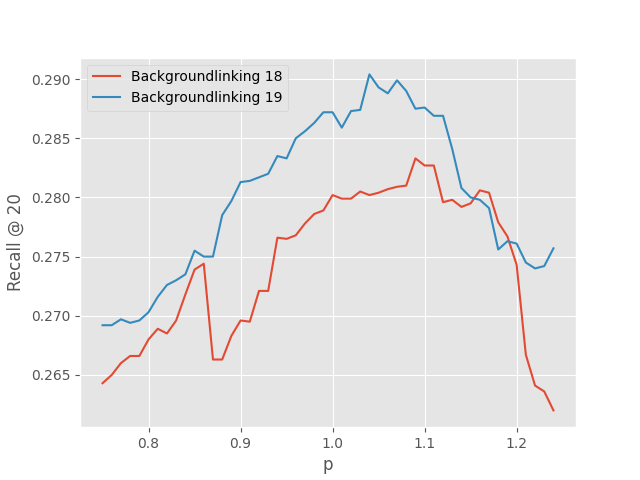
\includegraphics[width=0.9\linewidth]{./imgs/recall-20-geesedb.png}
	\caption{Recall @ 20 for varying levels of $p$}
	\label{geesedb-recall-20}
\end{figure}

\begin{figure}
	\centering
	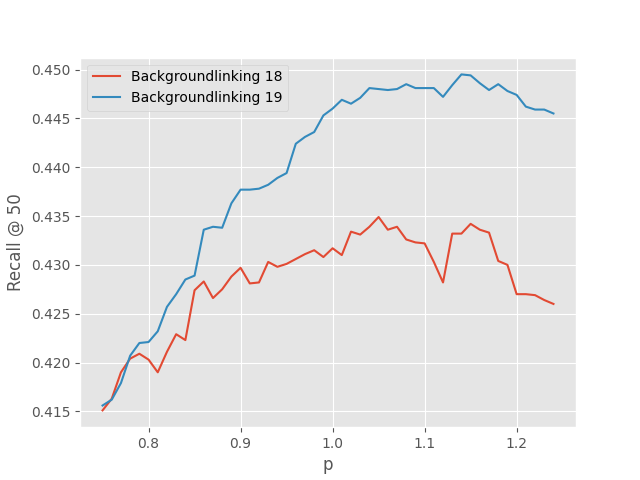
\includegraphics[width=0.9\linewidth]{./imgs/recall-50-geesedb.png}
	\caption{Recall @ 50 for varying levels of $p$}
	\label{geesedb-recall-50}
\end{figure}

\begin{figure}
	\centering
	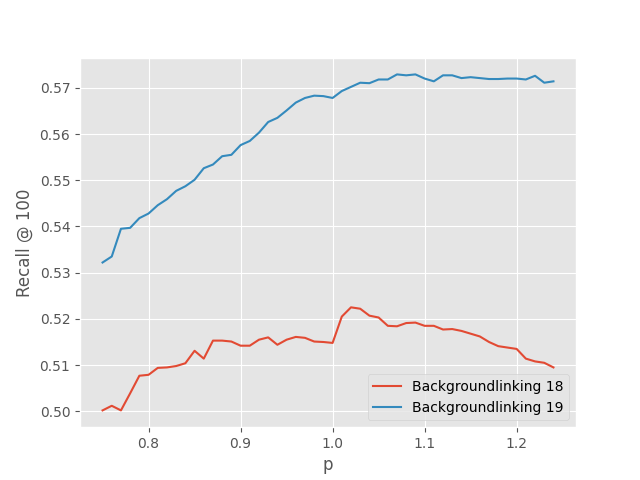
\includegraphics[width=0.9\linewidth]{./imgs/recall-100-geesedb.png}
	\caption{Recall @ 100 for varying levels of $p$}
	\label{geesedb-recall-100}
\end{figure}

\Cref{geesedb-recall-20,geesedb-recall-50,geesedb-recall-100} show the effectiveness scores for values of $p$ from $0.75$ to $1.25$ for recall at 20, 50 and 100. When $p = 1$, documents written by the same author get the same score. Values for $p$ lower than $1$ would decrease the scores for articles written by the same author.  
We see that for both collections, a slight boost of documents that are written by the same author, represented by the values $1 < p < 1.1$, does increase recall at different depths for both document collections.  However when $p$ becomes larger than $1.1$ the recall tends to decrease, especially for recall at depth $20$. 
This experiment shows that it is quite easy to use GeeseDB for retrieval experiments and adding metadata; showing that including metadata might benefit first stage ranking methods.

\section{Conclusion}
This chapter described the prototype implementation of GeeseDB, and how we envision graph databases be used for information retrieval research.
The GeeseDB system can be considered the answer on our research question: \emph{Can we extend the benefits from using relational databases for information retrieval to using graph databases, while being able to express graph-related problems easier?}
As GeeseDB is built on top of a relational engine it automatically inherits the benefits of using relational databases for IR. As GeeseDB can process graph queries, we also are able to express graph related problems. 

GeeseDB is still however a prototype system, and more functionalities need to be implemented. In particular, although the architecture is not coupled, it is not (yet) as efficient as traditional methods that do use coupled architectures. 

Not all graph operators have been supported in the current implementation. In order to make GeeseDB a usable system for IR researchers, more operators need to be implemented and the system needs to be developed to be more robust. 
 

\chapter{Creation of the Entity Graph}
\label{a-graph-of-entities}

\epigraph{``Is this new question a worthy one to investigate?'' This latter question we investigate without further ado, thereby cutting short an infinite regress.}{Alan Turing - 1950}


\begin{Abstract}
	\begin{changemargin}{1cm}{1cm}
		REBL is an extension of the Radboud Entity Linker (REL) for Batch Entity Linking. 
		REBL is developed after encountering unforeseen issues when trying to link the large MS MARCO v2 document collection with REL. In this chapter we discuss the issues we ran into and our solutions to mitigate them. REBL makes it easier to isolate the GPU heavy operations from the CPU heavy operations, by separating the mention detection stage from the candidate selection and entity disambiguation stages. By improving the entity disambiguation module we were able to lower the time needed for linking documents by an order of magnitude.
	\end{changemargin}
\end{Abstract}

\section{Introduction}
In the previous chapter we have introduced GeeseDB, a system that can query IR graphs and create rankings. We have used the system to express queries over the Washington Post news article collection. The examples we showed made use of entity annotations that were created by the Radboud Entity Linker (REL)~\citep{rel}.
Although, the Washington Post collection has been used for retrieval experiments, it is mostly used as a benchmark for news retrieval. 
In recent years, the MS MARCO ranking collections have become the de-facto benchmark for information retrieval experiments that employ deep learning. These collections are considerably larger than the Washington Post collection; the Washington Post collection consists of 728,626 news articles and blog posts, while the MS MARCO v2 document collections consists of almost 12 million web documents. The MS MARCO v2 document collections has almost 20 times as many documents, which are also longer on average.
When using REL, the Washington Post collection can be linked in a relatively short time. Using one GPU\footnote{NVIDIA GeForce RTX 3090} the linking time was amounted to approximately one day (24 hours). As the documents in the MS MARCO v2 document collection are longer than those in the Washington Post collection, we expected it would take about a month time to link this collection using the same system setup. As it is possible to divide the workload over multiple machines, the time needed to link all documents can be decreased easily by deploying more servers. 

When starting to link the first segment of this collection however, the time it took to link was considerably larger than expected. In fact, after 72 hours there was a time-out after only linking 20 percent of the segment (200k documents), a processing job that should only take about 12 hours (following a rough estimation). Why entity linking took so much more time than estimated by extrapolation was unclear. 

The goal of the research described in this chapter concerns our approach to understand and mitigate these efficiency issues, such that we could link the MS MARCO v2 document collection in an acceptable runtime. 
In databases runtime efficiency is often improved through set-at-a-time operations instead of tuple-at-a-time operations. This means that instead of doing all computations for one data entry at a time, one computation is calculated for all data entries, before starting the following computation. 

We investigate whether the set-at-a-time execution model from database research might be applicable in the context of entity linking as well. Specifically, we developed a batch extension for REL dubbed REBL. REBL splits different stages in entity linking such that partial computations for the whole dataset can be calculated before starting the next computation.
REBL improves REL efficiency by almost an order of magnitude, decreasing the processing time per document (excluding mention detection) on a sample of 5000 MS MARCO documents from 1.23 seconds to 0.13 seconds. Given modest computational resources, we demonstrate that REBL enables the annotation of a large corpus like MS MARCO v2. We discuss potential improvements that can be made to further improve batch entity linking efficiency. The REBL code and toolkit are available publicly at \url{https://github.com/informagi/REBL}.

Our third research question; 
\begin{itemize}
	\item \emph{Research Question 3: When does information retrieval research benefit from graph data?} 
\end{itemize} 
is not directly answered by the research described in this chapter. The research in this chapter was needed in order to obtain a dataset that we want to approach the third question. So, it forms the basis for the research described in the next chapter that will try to answers this question. In order to give proper context for the research described in this chapter, first entity linking will be described in more depth, before explaining the Radboud Entity Linking system that was used for this research. 

\section{Related Work}
Entity linking concerns identifying entity mentions in text and linking them to their corresponding entities in a knowledge graph. It fulfills a key role in the knowledge-grounded understanding of documents. It has been proven effective for diverse tasks in information retrieval~\citep{Gerritse:2022:EMBERT, Gerritse:2020:GEER, doc-ranking-entity, el-ranking-hasibi, el-balog, query-recommendation-entity, chatterjee2022bert}, natural language processing~\citep{lin-etal-2012-entity, watson}, and recommendation~\citep{yang-etal-2018-collective}.
% Maybe I should write out all these examples, if time permits. 
Utilizing entity annotations in these downstream tasks depends upon the annotation of text corpora with a method for entity linking. Due to the complexity of entity linking systems, this process is often performed by reliance on a third-party entity linking toolkit, where examples include DBpedia Spotlight~\citep{dbpedia-spotlight}, TAGME~\citep{tagme}, Nordlys~\citep{nordlys}, GENRE~\citep{genre}, Blink~\citep{blink}, and REL~\citep{rel}.

A caveat in existing entity linking toolkits is that they are not designed for batch processing large numbers of documents. Existing entity linking toolkits are primarily optimized to annotate individual documents, one at a time. This severely restricts utilizing state-of-the-art entity linking tools, such as REL, Blink, and GENRE, that employ neural approaches and require GPUs for fast operation. Annotating millions of documents incurs significant computational overhead, to the extent that annotation of a large text corpus becomes practically infeasible using modest computational power resources, especially when tagging documents one by one. Batch entity linking is, however, necessary to build today's data-hungry machine learning models, considering large text corpora like the MS MARCO v2 (12M Web documents)~\citep{msmarco}, or the newer ClueWeb22 collection~\citep{clueweb22}.

\section{REL}
This research specifically concerns the Radboud Entity Linking (REL) toolkit, in the context of processing large corpora. REL is a state-of-the-art entity linking system as shown emperically and independently by \citet{bast-etal-2023-fair}. Its system architecture is similar to that of competing systems, including BLINK~\citep{blink}.
REL annotates individual documents efficiently, requiring only modest computational resources while performing competitively compared to the state-of-the-art methods on effectiveness. It considers entity linking as a modular problem consisting of three stages:

\begin{itemize}
	\item \emph{Mention Detection.} 
	This step aims to identify all possible text spans in a document that might refer to an entity. If text spans that refer to entities are not appropriately identified, the system cannot correctly link the entity in later stages. REL is built to be a modular system, making it possible to use different named entity recognition (NER) systems for this stage. For REL the default system used is FLAIR, which is a state-of-the-art NER system that uses contextual word embeddings. 
	\item \emph{Candidate Selection.}
	For every detected mention, REL considers up to $k_1 + k_2 (=7)$ candidate entities. $k_1 (=4)$ candidate entities are selected based on their a priori occurrence probability $p(e|m)$ (for entity \textit{e} given mention \textit{m}). These priors are pre-calculated by summing Wikipedia hyperlinks and priors from the CrossWiki corpus~\citep{crosswiki}. The other $k_2 (=3)$ entities are chosen based on the similarity of their emtity embedding to the word embeddings of the context. In this stage, a context of a maximum of 200-word tokens is considered only.
	\item \emph{Entity Disambiguation.}
	The final step aims to map the mention to the correct entity in a knowledge base. The candidate entities for each mention are obtained from the previous stage. REL implements the Ment-norm method proposed by~\citet{ED-paper}.  
\end{itemize} 

After all entities have been found, REL produces a JSON object that contains the entities and their respective locations in the source text using standoff annotation. Because of REL's modular architecture, it is an ideal system to deploy set-at-a-time. 

\section{From REL to REBL}
The MS MARCO v2 document collection contains 11,959,635 documents split into 60 compressed files, totaling roughly 33GB. Uncompressed, these files are in JSON line format (where every line represents a document, described by a JSON object). These JSON objects have five fields: \textit{url}, \textit{title}, \textit{headings}, \textit{body}, and \textit{docid}. We wanted to link the documents' titles, headings, and bodies for our experiments. We link to the 2019-07 Wikipedia dump, one of the two dumps also used in the initial development of REL. It is, however, straightforward to take another dump of Wikipedia and deploy REL for that. 

In order to ease linking this size of data, we separated the GPU-heavy mention detection stage from the CPU-heavy candidate selection and entity disambiguation stages; the modified code can be found on GitHub.\footnote{\url{https://github.com/informagi/REBL} (last accessed -- October 27th, 2024)}
For REBL, the input for mention detection are the compressed MS MARCO v2 document files, and its output consists of the mentions found and their location in the document, in Apache Parquet format.\footnote{\url{https://github.com/apache/parquet-format} (last accessed -- May 8th, 2023)}
These files and the source text are the input for the subsequent phases (candidate selection and entity disambiguation). The final output consists of Parquet files containing spans of text and their linked entities. 
In the following section, we discuss what is changed for mention detection, candidate selection, and entity disambiguation steps to make REL more suited to annotate large collections with entity links, in a batch processing manner.  

\subsection{Mention Detection}
REL~\citep{rel} uses Flair~\citep{flair} as the default method for mention detection, a state-of-the-art named entity recognition system.
In this section, we focus on inefficiencies that arise when interfacing between REL and flair. 
Flair uses the \texttt{segtok}\footnote{\url{https://github.com/fnl/segtok}, (last accessed -- May 8th, 2023)} package to segment an (Indo-European) document in sentences, internally represented as \texttt{Sentence} objects. These sentences are split into words/symbols represented as \texttt{Token} objects.
When creating these representations, however, it is not possible to recreate the source text properly, as 
Flair adjusts the representations in its internal processing of text data. In order to have full control of these representations we decided to  construct the underlying data structures for REBL ourselves. To do this, we used the \texttt{syntok}\footnote{\url{https://github.com/fnl/syntok}, (last accessed -- May 8th, 2023)} package, a follow-up version of \texttt{segtok}.
Both packages were developed by the same author, who claims that the \texttt{syntok} package segments sentences better than \texttt{segtok}. 
Using this new representation we fixed two problems: 
\begin{enumerate}
	\item Flair removes white space characters when multiple occur after each other, REL accounts for this by counting the number of white spaces characters removed, a somewhat inefficient process prone to introduce inaccuracies in the mapping between source text and the annotated result. Using our own representation we know the start of every token, and we do not need an additional system that tracks the number of removed white spaces. So we change the interface between Flair and REL, as we create the Flair objects that REL uses manually. 
	\item Various zero width Unicode characters are removed by Flair from the source text before creating a token: zero width space (\texttt{U+200B}), zero width non-joiner (\texttt{U+200C}), variation selector-16 (\texttt{U+FE0F0}), and zero width no-break space (\texttt{U+FEFF}). 
	These characters occur rarely, but in a collection as large and diverse as MS MARCO v2, these characters do occur. When encountering these characters using REBL, the token objects were constructed such that the span and offset of the token still referred to that of the source text:
	For the case of the zero width space, we updated the \texttt{syntok} package. While, according to the Unicode standard, zero width space is not a whitespace character, it should be considered a character that separates two words. For the other Unicode characters removed by Flair, we manually update the span in the \texttt{Token} objects created by Flair such that they refer correctly to the positions in the source text. Now, when Flair identifies a series of tokens as a possible mention, we can directly identify the location in the source text from the \texttt{Token} objects.
\end{enumerate}

In order to efficiently use GPU resources, it is important to create batches of data to decrease the number of I/O operations. Every time a GPU calculation is called, data needs to be transferred from and to the GPU hardware. 
Flair does in fact support named entity recognition in batches; multiple pieces of text can be sent to the GPU, to achieve an overall faster inference time (as fewer I/O operations are needed). 
Because REL was designed to tag one document at a time, it did not utilize this functionality. REBL exploits this feature, allowing users to specify the number of documents to be tagged simultaneously, increasing linking efficiency. 

\subsection{Candidate Selection and Entity Disambiguation}
For candidate selection, REL makes use of a $p(e|m)$ prior, where \textit{e} is an entity, and \textit{m} is a mention. These priors are saved in an (SQLite) database, and up to 100 priors per mention are considered. However, data conversion between the client and the representation stored in the database incurred a high serialization cost. We updated this to a format that is faster to load, with the additional benefit of a considerably decreased database size.\footnote{The table that represents the priors shrank from $9.6$GB to $2.2$GB.}
We experimented with data storage in the DuckDB column-oriented database as an alternative. However, we found that SQLite was (still) more efficient as a key-value store, at least in DuckDB's state of development when we ran the experiments.

The entity disambiguation stage took much longer than reported in the original REL paper. This difference can partially be explained by the length of the documents to be linked. The documents evaluated by~\citet{rel} consisted of, on average, 323 tokens, with an average of 42 mentions to consider. The average number of tokens in an MS MARCO v2 document is about $1,800$, with 84 possible mentions per document.\footnote{These figures are calculated over the body field; we also tagged the shorter title and headers fields.}
Per mention, 100 tokens to the left and the right (so 200 total) are considered as context for the disambiguation model. 
The longer documents result in a higher memory consumption per context and document, with higher processing costs as the result.

We improve the efficiency of the entity disambiguation step such that it can be run in a manageable time. REL recreated a database cursor every time candidates where being generated. We rewrote the REL database code to create a single database cursor for the entity disambiguation module. 
When a mention occurs multiple times within a document, the exact same queries were issued to the database multiple times within a document.  By caching the output of these queries, we could considerably lower the number of database calls needed. We ended up caching all database calls for a segment, as we ran the process for every segment separately. 

The default setting of REL is to keep embeddings on the GPU after they are loaded, also ones that are not needed for disambiguation for following batches.
This design decision, however, slowed down disambiguation when many documents were being processed consecutively, because operations like normalization were carried out over all embeddings on the GPU. 
A considerable speed-up has been achieved by clearing these embeddings as soon as a document is processed.

Finally, after retrieving the embeddings from the database, REL puts them in a Python list. We rewrote the REL code such that the binary data is directly loaded from NumPy, a data format that Pytorch can use directly. 

\section{Effects on Execution}
In the mention detection stage, we improved tokenization and applied batching. The MS MARCO v1 collection does not contain characters that cause the problem in tokenization; the documents in that version of the collection were sanitized before it was published. In the MS MARCO v2 collection, $411,906$ documents have tokens that would be removed automatically by Flair, which corresponds to $3.4\%$ of all documents.
Batching documents in the mention detection stage decreased the average time for finding all named entities. We used batches of size 10, as the documents are relatively large. The optimal batch size will depend on the available GPU memory, and the length of the documents that need to be processed.

Some documents in the MS MARCO v2 collection cannot be linked. This happens only in extraordinary cases where linking with entities did not make sense in the first place, an example being a document consisting of numbers only. Here, the \texttt{syntok} package created one long \texttt{Sentence} object from this file that could not fit in GPU memory.

Table \ref{tab:efficiency} shows our improvements to the candidate selection and entity disambiguation step and describes how much time is saved in REBL. 
The code improvements to create the database cursor only once and to load the data directly from NumPy had no noticeable effect on the overall run time of entity disambiguation and are not reported in this table. This is likely because the costs of these operations are quite low, relatively to the efficiency improvements made by the other changes.
Note that the large standard deviations are primarily due to the differences in processing costs between long and short documents.

\begin{sidewaystable}
	\caption{Efficiency improvements for Candidate Selection and Entity Disambiguation. Improvements are calculated over a sample of 5000 documents using a machine with an Intel Xeon Silver 4214 CPU @ 2.20GHz using two cores with 187GB RAM and a GeForce RTX 2080 Ti (11GB) GPU. Improvements are cumulative; the times shown include the previous improvement as well.}
	\label{tab:efficiency}
	\begin{tabular}{p{6cm} c p{10cm}}
		\toprule
		Improvement & Seconds & Explanation\\
		\midrule
		Old Candidate Selection + Entity Disambiguation & $1.23 \pm 2.09$ & Average time it takes to select candidates and disambiguate per document\\
		\midrule
		No embedding reset & $0.26 \pm 1.60$ & The default setting of REL was to keep embeddings in GPU memory after they were loaded by clearing them from GPU memory after every document a speed up was achieved.\\
		Cache database calls & $0.15 \pm 1.31$ & When an entity occurs within a document, there is a high probability of it occurring multiple times. By caching the calls, we increase memory usage but can lower the time needed for candidate selection and entity disambiguation.  \\
		Representation change candidates & $0.13 \pm 1.19$ & By representing the candidates better in the database, we were able to save on conversion time, lowering the time needed for candidate selection.\\
		\bottomrule
	\end{tabular}
\end{sidewaystable}

\section{Conclusion and Discussion}
This chapter described REBL, an extension for the Radboud Entity Linker. We utilized REL's modular design to separate the GPU-heavy mention detection stage from the CPU-heavy candidate selection and entity disambiguation stages. The mention detection module is now more robust and reliable, using a better segmenter and preserving location metadata correctly.
The candidate selection and entity disambiguation steps were updated to improve their runtime Although it is now possible to run REL.~\citep{rel} on MS MARCO v2~\citep{msmarco} in a (for us) somewhat reasonable time, we identified further improvements to implement.

In the candidate selection step, found mentions are compared to all other mentions. The complexity of this step is $O(n^2)$, with $n$ being the number of mentions found in a document, which is especially problematic for longer documents. As we are only interested in similar mentions, it may be worthwhile to implement a locality-sensitive hashing algorithm to decrease the number of comparisons needed at this stage. 

Per mention, all context tokens are considered. This context has to be constructed from the source document. As a result, we load the source data a second time during candidate selection. Alternatively, we could output the mention context in the mention detection stage, which could speed up the candidate selection stage as we do not have to reconstruct the context for a second time. However, this would significantly increase the size of the mention detection output. More experiments are needed to strike the right balance here. 
Having a streaming approach would probably mitigate this issue. Another way a streaming approach might benefit REBL is that now, because a two-step approach is being used, intermediate results are written to the file system in parquet format. 

We have kept SQLite as the database backend but will consider specialized key-value stores to speed up candidate selection and entity disambiguation. Dedicated key-value stores probably can speed up those stages even more. 

Overall, it has become clear that a data processing-oriented perspective on entity linking is necessary for efficient solutions. A set-at-a-time approach should be preferred over a tuple-at-a-time approach when large amounts of data have to be processed. 
\chapter{MMEAD}
\label{ch:mmead}

\epigraph{The reader will have anticipated that I have no very convincing
	arguments of a positive nature to support my views. If I had I should not
	have taken such pains to point out the fallacies in contrary views.}{Alan Turing - 1950}

\begin{Abstract}
	\begin{changemargin}{1cm}{1cm}
		MMEAD, or MS MARCO Entity Annotations and Disambiguations, is a resource for entity links for the MS MARCO datasets. We specify a format to store and share links for both document and passage collections of MS MARCO. Following this specification, we release entity links to Wikipedia for documents and passages in both MS MARCO collections (v1 and v2). Entity links have been produced by the REL and BLINK systems. 
		MMEAD is an easy-to-install Python package, allowing users to load the link data and entity embeddings effortlessly. Using MMEAD takes only a few lines of code. Finally, we show how MMEAD can be used for IR research that uses entity information. We show how to improve recall@1000 and MRR@10 on more complex queries on the MS MARCO v1 passage dataset by using this resource. We also demonstrate how entity expansions can be used for interactive search applications. 
	\end{changemargin}
\end{Abstract}

\section{Introduction} 
The MS MARCO datasets~\citep{msmarco} have become the \emph{de facto} benchmark for evaluating deep learning methods for Information Retrieval (IR). The TREC deep learning track~\citep{trec-dl}, which has run since 2019, derives its datasets from the MS MARCO passage and document collections. The collections have been used in zero- and few-shot scenarios for diverse retrieval tasks and domains~\citep{thakur2021beir, thakur2022domain, xu2022laprador}. They also serve as primary resources for training deep learning models for downstream IR tasks such as conversational search~\citep{dalton2021cast} and search with knowledge graphs~\citep{Gerritse:2022:EMBERT} to achieve state-of-the-art results.

Purely text-based neural IR models, trained using MS MARCO collections, can generally not reason over complex concepts in the social and physical world~\citep{bosselut2021dynamic, sciavolino:2021:simple}. In response, recently proposed neuro-symbolic methods aim to combine neural models and symbolic AI approaches, e.g., by using knowledge graphs, which map concepts to symbols and relations. An essential step in developing neuro-symbolic models is connecting text to entities that represent the world's concepts formally. This step is mainly done using \textit{Entity linking}, an intermediary between text and knowledge graphs, which detects entity mentions in the text and links them to the corresponding entries in a knowledge graph.

Despite the proven effectiveness of neuro-symbolic AI -- and for IR models in particular~\citep{Tran:2022:DRE, Gerritse:2022:EMBERT, chatterjee2022bert} -- the IR community has made limited efforts to develop such models. A primary hindrance is the annotation of large-scale collections with entities; entity linking methods are computationally expensive. Running them over a large text corpus (e.g., MS MARCO v2 with 12M documents and 140M passages) requires extensive resources. This work aims to fill this gap by making entity annotations of the MS MARCO ranking collections readily available and easy to use. In the context of green AI / IR, computing the data only once, and then sharing it with many will reduce the amount of computation needed for people to carry out research on entity annotated web documents.

This chapter continues where the previous chapter ended. In the previous chapter the batch extension for the Radboud Entity Linking system, REBL, is introduced. In this chapter MMEAD is presented, a resource that provides entity links for the MS MARCO document and passage ranking collections. Two state-of-the-art entity linking tools, namely REL~\citep{rel}, with efficiency improvements made in REBL,~\citep{rebl} and BLINK~\citep{blink}, are utilized for annotating the corpora. The annotations are stored in a DuckDB database, enabling efficient analytical operations and fast access to the entities. The resource is available as a Python package and can be installed from PyPI effortlessly. The resource also includes a sample demo, enabling queries with complex compositional structures about entities. 

The primary objective of the work in this chapter is to simplify the study of neuro-symbolic IR research, enabling further steps in neural IR. In our experiments, we show significant improvements on recall for neural re-ranking IR models when using MMEAD annotations as bag-of-word expansions for queries and passages. Our experiments reveal that the difference in effectiveness is even greater (in terms of both recall and MRR) for complex queries that require further reasoning over entities.

To show the usefulness of our resource beyond plain ranking, we also present how to enrich interactive search applications. Specifically, we demonstrate how to obtain entities' geographical locations by relating the entities found in passages to their Wikidata entries. Plotting these entities on the world map shows that the MS MARCO passages can be geo-located all over the world.
We can also move from location to web text by retrieving all passages associated with a geographical location.

To return to our last research question; 
\begin{itemize}
	\item \emph{Research Question 3: When does information retrieval research benefit from graph data?} 
\end{itemize}   
This chapter attempts to demonstrate that graph data, in this case a graph of entities, can help retrieval by considering metadata that is included through graph operations. Although we have not used GeeseDB, the work described in~\cref{from-tables-to-graphs}, it would be a natural application of GeeseDB to carry out the query expansion methods described.

In summary, this chapter makes the following contributions:
 \begin{itemize}
	\item We annotate the documents of the MS MARCO passage and document collections and share these annotations. By sharing these annotations, we ease future research in neuro-symbolic retrieval, which extensively uses entity information. We also provide useful metadata such as Wikipedia2Vec~\citep{wikipedia2vec} entity embeddings. 
	\item We provide a Python library that makes our data easy to use. All data is stored in DuckDB tables, which can be loaded and queried quickly. The library is easy to install through PyPI, and the entity annotations are available with only a few lines of code.
	\item We experimentally show that retrieval effectiveness measured by recall significantly increases when using MMEAD. The improvement is even greater for complex queries, where we observe low retrieval effectiveness using text-only IR models.
	\item We demonstrate how the data can be used in geographical applications. For example, we can plot on a static map all entities found in the MS MARCO v2 passage collection for which geographical data is available. Additionally, one can retrieve all passages associated with a geographical location.  
\end{itemize}

MMEAD is publicly available at \url{https://github.com/informagi/mmead}.

\section{Background}
In this section, we describe systems that are used for creating entity annotations on the MS MARCO collections for MMEAD. Some information presented in this section overlaps with that of the previous chapter, but the full context is included here to enable reading this chapter as standalone work.

\subsection{REL}
REL (Radboud Entity Linker)~\citep{rel} is a state-of-the-art open-source entity linking tool designed for high throughput and precision. REL links entities to a knowledge graph (Wikipedia) using a three-stage approach: (1) mention detection, (2) candidate selection, and (3) entity disambiguation. We briefly explain these three steps:

\begin{enumerate}
	\item \emph{Mention Detection.} REL starts the entity linking process by first identifying all text spans that might refer to an entity. In this stage, it is essential that all possible entities in the text are identified, as only the output of this stage can be considered an entity by REL. These spans are identified using a named entity recognition (NER) model based on contextual word embeddings. For our experiments, we use the NER model based on Flair~\citep{flair} embeddings. 
	\item \emph{Candidate Selection.} Up to seven candidate entities are considered for every mention found by Flair. Part of these entities are selected according to the prior probability $P(e|m)$ of the mention $m$ being linked to the entity $e$. This probability is estimated from existing dictionaries YAGO~\citep{yago}, Wikipedia, and CrossWikis~\citep{crosswiki}. Precisely, the top-4 ranked entities are selected based on $P(e|m) = \min(1, P_{\mathit{Wiki}}(e|m) + P_{\mathit{YAGO}}(e|m))$, where $P_{\mathit{YAGO}}(e|m))$ is a uniform probability from the YAGO dictionary and $P_{\mathit{Wiki}}(e|m)$ is computed based on the summation of hyperlink counts in Wikipedia and the CrossWikis corpus.
	%, and a uniform probability from the YAGO dictionary~\citep{yago}. These probabilities are precalculated for every mention: $P(e|m) = \min(1, P_{\mathit{Wiki}}(e|m) + P_{\mathit{YAGO}}(e|m))$.
	The remaining three candidate entities are determined according to the similarity of an entity and the context of a mention. For the top-ranked candidates based on $P(e|m)$ probabilities, the context similarity is calculated by $\mathbf{e}^T \sum_{w\in c}\mathbf{w}$. Here $\mathbf{e}$ is the entity embedding for entity $e$, and $\mathbf{w}$ are the word embeddings in context $c$, with a maximum length of 200-word tokens. The entity and word embeddings are jointly learned using Wikipedia2Vec~\citep{wikipedia2vec}. 
	\item \emph{Entity Disambiguation.} The final stage tries to select the correct entity from the candidate entities and maps it to the corresponding entry in a knowledge graph (Wikipedia). For this, REL assumes a latent relation between entities in the text and utilizes the Ment-norm method proposed by~\citet{ED-paper}.
\end{enumerate}

\subsection{BLINK}
BLINK~\citep{blink} is a BERT-based~\citep{BERT} model for candidate selection and entity disambiguation, which assumes that entity mentions are already given. When utilized in an end-to-end entity linking setup, BLINK achieves similar effectiveness scores as REL. Below we describe the three steps of mention detection, candidate selection, and entity disambiguation for end-to-end entity linking using BLINK.

\begin{enumerate}
    \item \emph{Mention Detection.} The mention detection stage can be done using an NER model. Like REL, we use Flair~\citep{flair} for mention detection.
	\item \emph{Candidate Selection.} BLINK considers ten candidates for each mention. The candidates are selected through a bi-encoder (similar to the bi-encoder described by~\citet{poly-encoders}) that embeds mention contexts and entity descriptions. The mention and the entity are encoded into separate vectors using the \texttt{[CLS]} token of BERT. The similarity score is then calculated using the dot-product of the two vectors representing the mention context and the entity.  
	\item \emph{Entity Disambiguation.} For entity disambiguation, BLINK employs a cross-encoder to re-rank the top 10 candidates selected by the candidate selection stage. The cross-encoder usage is similar to cross encoder described by~\citet{poly-encoders}, which employs a cross-attention mechanism between the mention context and entity descriptions. The input is the concatenation of the mention text and the candidate entity description.    
\end{enumerate}

\subsection{DuckDB}
DuckDB~\citep{duckdb} is an in-process column-oriented database management system. It is designed with requirements that are beneficial for the MMEAD resource:
\begin{enumerate}
    \item \emph{Efficient analytics.} DuckDB is designed for analytical (OLAP) workloads, while many other database systems are optimized for transactional queries (OLTP). DuckDB is especially suitable for cases where analytics are more important than transactions. As we release a resource, transactions (after loading the data) are unnecessary, making an analytics database more useful than a transactional-focused one.  
	\item \emph{In-process.} DuckDB runs in-process, which means no database server is necessary, and all data processing happens in-process. This allows the database to be installed from PyPI without any additional steps. 
	\item \emph{Efficient data transfer.} Because DuckDB runs in-process, it can transfer data from and to the database more easily, as the address space is shared. In particular, DuckDB uses an API built around NumPy and Pandas, which makes data (almost) immediately available for further data analysis within Python. 
\end{enumerate}
DuckDB also supports the JSON and parquet file formats, making data loading especially fast when data is provided in such formats.

\section{MMEAD}
MMEAD provides links for MS MARCO collections v1 and v2 created by the REL entity linker, and links for the MS MARCO v1 passage collection by the BLINK entity linker. For REL, we use its batch entity linking extension, REBL~\citep{rebl}. The knowledge graphs used for the REL and BLINK entity linkers are Wikipedia dumps from 2019-07 and 2019-08, respectively. Both dumps are publicly available from the linking systems' Github pages. 

\subsection{Goals}
The design criteria for MMEAD are based on the following goals:
\begin{itemize}
    \item \emph{Easy-to-use.} It should be easy to load and use the linked entities in experiments. With only a few lines of code, it should be possible to load entities and use them for analysis. Additional information should also be readily available, like where entities appear in the text and their latent representations.
	\item \emph{High-quality entity links.} We wish to release high-quality entity links for the MS MARCO collections, so that applying neuro-symbolic models and reasoning over entities becomes feasible.
	\item \emph{Extensibility.} It should be easy to link the collections with a different entity linking system and publish them in the same format as MMEAD. This way, we can integrate links produced by other entity linking systems and make them automatically available through the MMEAD framework.
	\item \emph{Useful metadata.} Additional data that can help with experiments should be provided; this includes mapping entities to their respective identifiers and latent representations.  
\end{itemize}

\subsection{Design}
\paragraph{Easy-to-use.} To create an easy-to-use package, we make the MMEAD data publicly available as JSONL files, which is the same format as the MS MARCO v2 collections. Each line of JSON contains entity links for one of the documents or passages in the collections; see Figure~\ref{fig:json-example-passage-v1}. The corresponding document can be identified through the JSON field that represents the document/passage identifier: \texttt{docid} for documents and \texttt{pid} for passages. Then, for every section of a document, a separate JSON field is available to access the entities in that section. For passages, there is only one section containing the entity annotations of the passage, while for MS MARCO v2 documents, we link not only the \texttt{body} of the document but also the \texttt{header} and the \texttt{title}.

All essential information about the entity mentions and linked entities is stored in the JSON objects. 
Specifically, the following metadata is made available: \texttt{entity\_id}, \texttt{start\_pos}, \texttt{end\_pos}, \texttt{entity}, and \texttt{details}. The field \texttt{entity\_id} stores the identifier that refers to the entry in the knowledge graph (Wikipedia, in our case). The \texttt{start\_pos} and \texttt{end\_pos} fields store the start and end positions of the text span that refers to the linked entity (i.e., as a standoff annotation of the entity mention). The positions are UTF-8 indices into the text, ready to be used in Python to extract the relevant parts of the document. The field \texttt{entity} stores the text representation of the entity from the knowledge graph. 
We chose to store this field for convenience and human readability. The \texttt{details} field is a JSON object that stores linker-specific information; examples include the entity type according to the NER module and the confidence of the identified mention.

\paragraph{High-quality entity links.} MMEAD provides entity links produced by state-of-the-art entity linking systems. Both REL and BLINK are high precision entity linkers, ensuring that identified mentions and their corresponding entities are likely correct. The knowledge graphs used by the entity linkers are the same as those used in the original studies; this way, extensive research has been done to confirm the precision of the linking systems.

\paragraph{Extensibility.} We ensure extensibility by clearly describing the format in which the entity links are provided. If another system shares its links in the same format, the MMEAD Python library can work with the data directly. The \texttt{details} field per entity annotation enables inclusion of linker-specific information. REL provides specific instructions on updating the system to newer versions of Wikipedia in its documentation, making it possible to easily release links to newer versions of Wikipedia.

\paragraph{Useful metadata.} Alongside the entity links, we also provide additional useful metadata. Specifically, we release Wikipedia2Vec~\citep{wikipedia2vec} embeddings (300d and 500d feature vectors). REL uses the 300d Wikipedia2Vec feature vectors internally for candidate selection. These feature vectors consist of word embeddings \emph{and} entity embeddings mapped into the same high-dimensional feature space. These embeddings can be used directly for information retrieval research~\citep{Gerritse:2020:GEER, Gerritse:2022:EMBERT}. We also release a mapping of entities to their identifiers. The entity descriptions can change in different versions of Wikipedia, but their identifiers remain constant.
The identifier can also be used to find the corresponding entity in other knowledge graphs such as Wikidata.

\subsection{An Example}
A passage from the MS MARCO v1 passage ranking collection is shown below.\footnote{This is the second passage from the collection.}

\smallskip
\begin{center}
	\fbox{
		\begin{minipage}{0.9\textwidth}
			\emph{The Manhattan Project and its atomic bomb helped bring an end to World War II. Its legacy of peaceful uses of atomic energy continues to have an impact on history and science.}
		\end{minipage}
	}    
\end{center}
\smallskip

A few text spans in this text can be considered as entities: ``the Manhattan Project'', ``World War II'', and ``atomic energy.'' REL identifies two of these entities: the \emph{Manhattan Project} and \emph{World War II}. 
The output of the system is converted to our JSON specification, which results in the JSON object presented in Figure~\ref{fig:json-example-passage-v1}. The value of the \texttt{md\_score} field shows that Flair is more certain about ``World War II'' being an entity than the ``Manhattan Project.'' 

\begin{figure}
	\begin{minted}[]{json}
{
	"passage": [
	{
		"entity_id": 19603, 
		"start_pos": 4, 
		"end_pos": 21,
		"entity": "Manhattan Project",
		"details": {
			"tag": "ORG",
			"md_score": 0.613243
		}
	}, 
	{
		"entity_id": 32927,
		"start_pos": 65,
		"end_pos": 77,
		"entity": "World War II",
		"details": {
			"tag": "MISC",
			"md_score": 0.991474
		}
	}
	], 
	"pid": 1
}
	\end{minted}
\caption{Example of MMEAD annotations for a MS MARCO passage in JSON format. The field \texttt{tag} depicts the type of the entity and \texttt{md\_score} shows the certainty of the mention detection component in identifying the text span as a mention.}
\label{fig:json-example-passage-v1}
\end{figure}

Table~\ref{number-links} shows the number of entities found in the collections by the REL system. Blink found 21,968,356 entity links for the v1 passage collection.  For 11,177,904 entities, the two linking systems produced exactly the same output. 

\begin{table}
\centering
\caption{Number of entities linked by REL; we show the total number of entities found and how many entities there are per passage/document on average.}
\begin{tabular}{c|c|c}
	\toprule
	& passages & docs \\
	\midrule
	MS MARCO v1 & 18,561,221 (2.10) & 145,725,732 (45.34) \\
	MS MARCO v2 & 233,254,024 (1.69) & 661,183,287 (55.28) \\
	\bottomrule
\end{tabular}
\label{number-links}
\end{table}

\section{How To Use}

MMEAD comes with easy-to-use Python code, allowing users to work with the resource effortlessly. To start, MMEAD can be installed from PyPI using pip:

\begin{verbatim}
$ pip install mmead
\end{verbatim}

After installation, the entity links can be loaded into a DuckDB database~\citep{duckdb}, as shown in Figure~\ref{fig:load-links}, with only a couple of lines of code.
%
\begin{figure}
\begin{minted}[linenos]{python}
from mmead import get_links
links = get_links('v1', 'passage', linker='rel')
\end{minted}
\caption{Example of how to load MMEAD entity links for the MS MARCO v1 passage collection.}
\label{fig:load-links}
\end{figure}
%
When running this code for the first time, initialization will take some time, as all the data need to be downloaded and ingested into the DuckDB database. After loading the data for the first time, it is automatically stored on disk. Loading the persisted data for later usage will only take seconds.

Once the data is loaded, it is ready to use. We provide a simple interface to access the data. The code shown in Figure~\ref{fig:load-links-for-document} loads the entity links available for a document in the MS MARCO v1 passage ranking collection. When using this function, the data is provided in JSON format, making it easy to access the annotations.

\begin{figure}
\begin{minted}[linenos]{python}
>>> links.load_links_from_docid(123)
{"passage":[{"entity_id":"7954681", ... }
\end{minted}
	\caption{Example of how to load the entity links for a document. For formatting reasons, we do not show the full output. }
	\label{fig:load-links-for-document}
\end{figure}

We also provide word embeddings and entity embeddings generated by Wikipedia2Vec~\citep{wikipedia2vec} based on the 2019-07 Wikipedia dump. These embeddings are stored in DuckDB tables and are available as Numpy arrays after loading. Figure~\ref{fig:dot-product} shows how embeddings are loaded using MMEAD. The example demonstrates that the entity embedding of \emph{Montreal} and the word embedding of ``Montreal'' are closer to each other than the word embeddings of the two words ``Montreal'' and ``green'' based on dot-product as a similarity function. The dimensionality of the embedding vectors (300 or 500) can be specified in the code.

\begin{figure}
	\begin{minted}[linenos]{python}
>>> from mmead import get_embeddings
>>> e = get_embeddings(300, verbose=False)
>>> montreal_word = e.load_word_embedding("Montreal")
>>> montreal_entity = e.load_entity_embedding("Montreal")
>>> green_word = e.load_word_embedding("green")

>>> montreal_word @ montreal_entity
31.83191792
>>> montreal_word @ green_word
5.55568354

>>> toronto_word = e.load_word_embedding("Toronto")
>>> toronto_word
array([-1.497e-01, -7.765e-01, -1.000e-02, ...])
>>> montreal_word @ toronto_word
21.62585146
	\end{minted}
	\caption{Example code for loading word and entity embeddings. It shows that the dot-product between ``Montreal'' word and entity embeddings is greater than the dot-product of embedding vectors for the word ``Montreal'' and ``green'' (a word chosen at random). The word embeddings of Montreal and Toronto, two cities in Canada, are also more similar.}
	\label{fig:dot-product}
\end{figure}

The mapping between the official Wikipedia identifiers and entity text representations is extracted from the 2019-07 Wikipedia dump. If entity annotations from another version of Wikipedia are available, the MMEAD mappings can be used to match entities between the dumps. 
Needless to say, emerging entities in newer versions of Wikipedia cannot be mapped to the version that is available in MMEAD. However, existing entities in MMEAD can be mapped to newer versions of Wikipedia in a straightforward manner.
Figure~\ref{fig:load_mappings} shows how entity identifiers can be matched to their text and the other way around.  

\begin{figure}
	\begin{minted}[linenos]{python}
>>> from mmead import get_mappings
>>> m = get_mappings(verbose=False)
>>> m.get_id_from_entity('Montreal')
7954681
>>> m.get_entity_from_id(7954681)
'Montreal'
	\end{minted}
	\caption{Entity names and identifiers are accessible in MMEAD. Given an entity text, we can directly find its corresponding identifier and vice versa.}
	\label{fig:load_mappings}
\end{figure}

As DuckDB is used as a database engine for MMEAD, it is possible to directly access the underlying tables and issue structured queries in an efficient manner. Figure~\ref{fig:sql_engine} shows an example, where a connection to the database is created, and the identifiers of passages containing the entity \emph{Nijmegen} are retrieved.

All data can be downloaded directly as well, and links to the data are provided on our Github page.\footnote{\url{https://github.com/informagi/mmead}, last accessed November 18th 2024}

\begin{figure}
	\begin{minted}[linenos]{python}
>>> from mmead import load_links
>>> cursor = load_links(
...     'msmarco_v1_passage_links',
...     verbose=False
... )
>>> cursor.execute("""
...     SELECT pid 
...     FROM msmarco_v1_passage_links_rel 
...     WHERE entity='Nijmegen'
... """)
[(771129,), (1273612,), (1418035,), ... ]
	\end{minted}
	\caption{All data is stored in DuckDB tables, and thus it is possible to directly access the tables and issue queries. In this example, we extract the identifiers of passages that contain the city of Nijmegen.}
	\label{fig:sql_engine}
\end{figure}

\section{Entity Expansion with MMEAD}
To demonstrate the usefulness of MMEAD for (neural) retrieval models, we have conducted experiments that extend existing models with MMEAD annotations.
These experiments serve a demonstrative purpose only, and the full potential of this resource is to be further explored in (neuro-)symbolic IR models~\citep{Gerritse:2022:EMBERT,Tran:2022:DRE}.

\subsection{Methods}

\paragraph{BM25 expansion.} We experimented with three retrieval methods to show the benefits of entity annotation for passage ranking: one baseline method and two methods that use query entity expansion~\citep{Shehata} using REL:

\begin{itemize}
	\item[\textbf{a}] \textbf{BM25 -- No Expansion.} As a baseline method, we used BM25 as implemented in Anserini~\citep{anserini} using hyper-parameters $k_1=0.82$ and $b=0.68$, shown to be optimal for the MS MARCO dataset. MS MARCO was indexed normally, and no expansion was considered for the queries or the passages. 
	\item[\textbf{b}] \textbf{BM25 -- Entity Text Expansion.} In this method, passages and queries are expanded with the text representation of their annotated entities (from REL). Once the passages and queries have been expanded with entities, we run BM25 with the same hyper-parameter settings as described in \textbf{a}.
	\item[\textbf{c}] \textbf{BM25 -- Entity Hash Expansion.} Instead of using the text representation of entities as an expansion, we expanded the passages and queries by the MD5 hash of the entity text (from REL). The use of MD5 hashing provides a consistent representation of multi-word terms and avoids partial or incorrect matching between queries and non-relevant passages; e.g., passages that contain the word ``united'', do not benefit if the query contains ``United States'' as an entity. Again, after expansion, we run BM25 with the same hyper-parameter settings described in \textbf{a}.
\end{itemize}
In these experiments, the identified entities are deduplicated. As a demonstration of the proposed text expansion methods, Figure~\ref{fig:exp_queries} shows how the query expansion is performed using explicit and hashed forms. The added entities provide more precise context and help eliminate ambiguous terms. Figure~\ref{fig:exp_passage} shows the expansion methods on the relevant passage for this query. The relevant passage can be found through our expansion technique. The linking system recognizes that both the query and the passage contain a reference to the entity \emph{Sacagawea}, even though they are spelled differently in the query and the passage.

\begin{figure}
	\framedtext{
		\begin{itemize}
			\item[\textbf{a.}] did sacajawea cross the pacific ocean with lewis and clark
			\item[\textbf{b.}] \underline{The same text as shown in \textbf{a.}} + \emph{Sacagawea} \emph{Clark} \emph{Pacific Ocean} \emph{C. S. Lewis}
			\item[\textbf{c.}] \underline{The same text as shown in \textbf{a.}} + \texttt{860324} \texttt{a97fed} \texttt{3e3b0e} \texttt{3fe907}
		\end{itemize}
	}
	\caption{Examples of queries for the three different experiments; (\textbf{a}) the non-expanded query, (\textbf{b}) the query with entity text expansion, and (\textbf{c}) the query with entity hash expansion. Text expansions are shown in italics. The MD5 hashes shown in (\textbf{c}) are shortened for formatting.}
	\label{fig:exp_queries}
\end{figure}

\begin{figure}
	\framedtext{
		\begin{itemize}
			\item[\textbf{a.}] Introduction. Sacagawea, as everyone knows, was the young Indian woman who, along with her baby, traveled with Lewis and Clark to the Pacific Ocean and back.She was a great help to the expedition and many organizations are preparing celebrations to commemorate the 200-year anniversary of the endeavor.y: M. R. Hansen. Sacagawea, as everyone knows, was the young Indian woman who, along with her baby, traveled with Lewis and Clark to the Pacific Ocean and back.
			\item[\textbf{b.}] \underline{The same text as shown in \textbf{a.}} + \emph{Indian Ocean} \emph{James Hansen} \emph{Sacagawea} \emph{India} \emph{Oceania} \emph{William Clark} \emph{Meriwether Lewis} \emph{Pacific Ocean}
			\item[\textbf{c.}] \underline{The same text as shown in \textbf{a.}} + \texttt{fe6fc8} \texttt{860324} \texttt{aa84e6} \texttt{7847ef} \texttt{3e3b0e} \texttt{7d31e0} \texttt{2d8836} \texttt{e58bef}
		\end{itemize}
	}
	\caption{The relevant passage for the query presented in Figure~\ref{fig:exp_queries}; (\textbf{a}) the non-expanded passage, (\textbf{b}) the passage with entity text expansion, and (\textbf{c}) the passage with entity hash expansion. Text expansions are in italics. The MD5 hashes shown in (\textbf{c}) are shortened for formatting.}
	\label{fig:exp_passage}
\end{figure}


\paragraph{Reciprocal Rank Fusion.} As a second series of experiments, we applied Reciprocal Rank Fusion (RRF)~\citep{10.1145/1571941.1572114} to the runs described above. RRF is a fusion technique that can combine rankings produced by different systems. RRF creates a new ranking by only considering the rank of a document in the input. Given a set of documents $D$ and a set of rankings $R$, RRF can be computed as: 
\begin{equation}
	\mathit{RRF}(d \in D) = \sum_{r\in R}\frac{1}{k + r(d)}
\end{equation}
Here $k$ is a hyperparameter that can be optimized, but we simply used a default value of $k=60$ for all settings.

This provides us with four new rankings; the RRF of the pairwise combinations of the three rankings described above and the RRF of all three of these runs:
\begin{itemize}
	\item[\textbf{d.}] \textbf{RRF -- No Expansion + Entity Text.} RRF fusion of runs \textbf{a} and \textbf{b}. The run with no expansions and the run with entity text expansions are considered.
	\item[\textbf{e.}] \textbf{RRF -- No Expansion + Entity Hash.} RRF fusion of runs \textbf{a} and \textbf{c}. The run with no expansions and the run with entity hash expansions are considered.
	\item[\textbf{f.}] \textbf{RRF -- Entity Text + Entity Hash.}  RRF fusion of runs \textbf{b} and \textbf{c}. The run with entity text expansions and the run with entity hash expansions are considered.
	\item[\textbf{g.}] \textbf{RRF -- No Expansion + Entity Text + Entity Hash.} RRF fusion of runs \textbf{a}, \textbf{b}, and \textbf{c}. All three runs are considered. 
\end{itemize}

\subsection{Experimental Setup}
In our experiments, we use MMEAD as a resource to expand queries and passages with entities. The experiments are performed using the MS MARCO v1 passage ranking collection, where only queries containing at least one entity annotation are used. We do not expect meaningful differences for queries without any linked entities, as the expanded query is identical to the original query in that case. 

As we expect the linked entities to provide additional semantic information about the queries and passages, we conduct further testing on the obstinate query sets of the MS MARCO Chameleons~\citep{chameleons}, which consist of challenging queries from the original MS MARCO passage dataset. In general, ranking methods show poor effectiveness in finding relevant matches for these queries. Our testing focuses on the bottom 50\% of the worst-performing queries from the subsets of Veiled Chameleon (Hard), Pygmy Chameleon (Harder), and Lesser Chameleon (Hardest), which represent increasing levels of difficulty. 

This gives us four query sets on which we evaluate; (1) all queries that contain entity annotations (\emph{dev} -- 1984 queries), (2) all queries in the hard subset that contain entity annotations (\emph{hard} -- 680 queries), (3) all queries in the harder subset that contain entity annotations (\emph{harder} -- 493 queries), and lastly, (4) all queries in the hardest subset that have entity annotations (\emph{hardest} -- 322 queries).

The experiments are evaluated using Mean Reciprocal Rank (MRR) at rank ten and Recall (R) at rank one thousand. MRR@10 is the official metric for the MS MARCO passage ranking task, while R@1000 gives an upper limit on how well re-ranking systems could perform. The Anserini~\citep{anserini} toolkit is used to generate our experiments. 

\subsection{Results}

\begin{sidewaystable}
		\centering
		\caption{Results on the MS MARCO v1 passage collection, using only the queries that have entity annotations. Bolded numbers are the highest achieved effectiveness. Scores with a dagger (\dag) are significantly better compared to BM25 with no expansion (run \emph{a}), following a paired t-test with Bonferroni correction. For MRR, we have not calculated significance scores due to its ordinal scale~\citep{fuhr-mrr}.}
		\tabcolsep=0.11cm
		\begin{tabular}{rll|llll|llll}
			\toprule
			\multirow{2}{*}{}
			& & & \multicolumn{4}{c|}{R@1000} & \multicolumn{4}{c}{MRR@10} \\
			& & & \multicolumn{1}{c}{dev} & \multicolumn{1}{c}{hard} & \multicolumn{1}{c}{harder} & \multicolumn{1}{c|}{hardest} & \multicolumn{1}{c}{dev} & \multicolumn{1}{c}{hard} & \multicolumn{1}{c}{harder} & \multicolumn{1}{c}{hardest} \\
			\midrule
			a. & BM25 & No Expansion                       & 0.9111 & 0.7855 & 0.7444 & 0.6677 & \textbf{0.2413} & 0.0373 & 0.0137 & 0.0000 \\
			b. & BM25 & Entity Text                        & 0.9183 & 0.8240\dag & 0.7951\dag & 0.7298\dag & 0.2202 & 0.0385 & 0.0173 & \textbf{0.0057} \\
			c. & BM25 & Entity Hash                        & 0.9105 & 0.7980 & 0.7576 & 0.6848 & 0.2199 & 0.0383 & \textbf{0.0175} & 0.0052 \\ \midrule
			\multirow{2}{*}{}
			d. & RRF & No Expansion          & \textbf{0.9338}\dag & \textbf{0.8436}\dag & \textbf{0.8124}\dag & \textbf{0.7500}\dag & 0.2372 & 0.0385 & 0.0163 & 0.0019 \\
			& & + Entity Text &&&&&&&& \\
			\multirow{2}{*}{}
			e. & RRF &  No Expansion     & 0.9250\dag & 0.8260\dag & 0.7921\dag & 0.7205\dag & 0.2378 & 0.0367 & 0.0152 & 0.0034 \\
			&&  + Entity Hash  &&&&&&&& \\
			f. & RRF & Entity Text \& Hash                 & 0.9231 & 0.8260\dag & 0.7982\dag & 0.7314\dag & 0.2218 & 0.0375 & 0.0161 & 0.0053 \\
			\multirow{2}{*}{}
			g. & RRF & No Expansion   & 0.9313\dag & 0.8370\dag & 0.8043\dag & 0.7376\dag & 0.2358 & \textbf{0.0391} & 0.0156 & 0.0035 \\
			&& + Entity Text \& Hash &&&&&&&& \\
			\bottomrule 
		\end{tabular}
		\label{tab:results-table}
\end{sidewaystable}

Table~\ref{tab:results-table} presents the results of our experiments. If we first look at lines \textbf{a-c} in the results table, we can examine the effects of our expansion methods compared to the baseline run. Looking at R@1000, we can see that more relevant passages are found using entity expansion for the \emph{dev} collection and its harder subsets. We do not find additional relevant documents/passages on the \emph{dev} set when we use the entity hashes, and entity text seems to be the better approach. There is, however, no increase in MRR@10 when using this expansion method. Entity expansions help when evaluating using R@1000, especially when the queries are more complex. The difference in recall effectiveness becomes larger the more complex the queries get. MRR@10 only improves when using entity text expansion.

The reciprocal rank fusion methods are presented in lines \textbf{d-g}. When using these methods, the R@1000 increases more. Again, the subsets that contain more complex queries tend to benefit more. Regarding R@1000 effectiveness, the best RRF method uses a ranking from the normal, not expanded index, with the index that has been expanded with the entity text. Again, entity text expansion helps recall more than using hash expansion. Although the RRF methods improve recall, MRR@10 does not benefit from RRF when compared to using only one of the expansion techniques. 

\section{Beyond Quantitative Results}
In the previous section, we demonstrated the potential value of MMEAD using quantitative evaluations, where we leverage entities to improve retrieval effectiveness in standard benchmark datasets.
Beyond these quantitative results, MMEAD can also help enrich interactive search applications in various ways.
This section describes a few such examples.

\begin{figure}
	\centering
	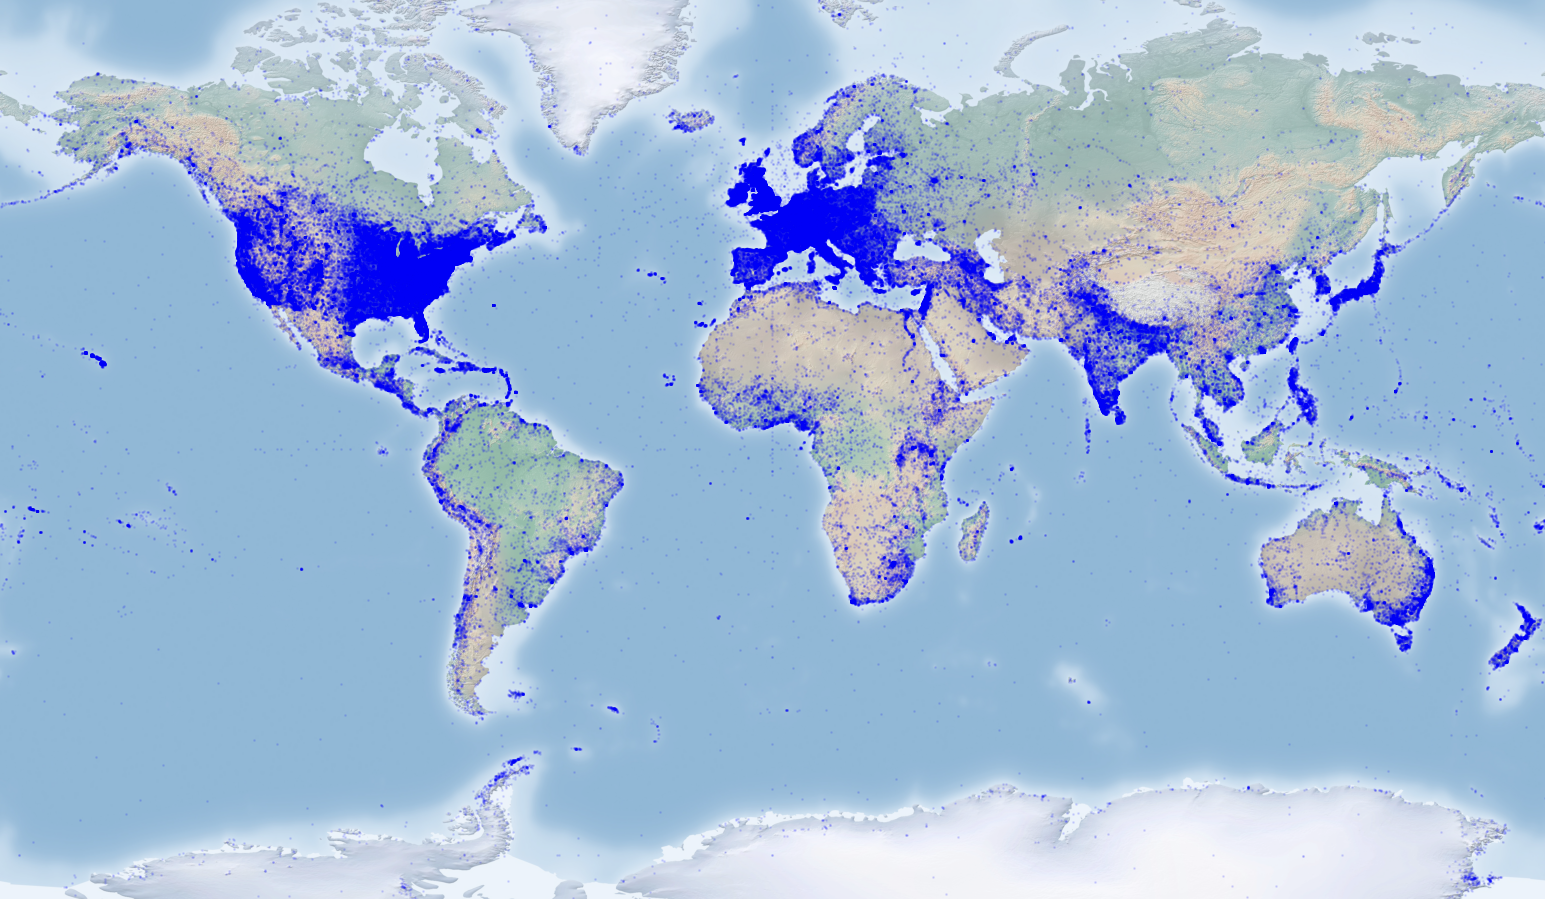
\includegraphics[width=.9\textwidth]{imgs/basemap_shaded_blue_opa.png}
	\caption{Locations of entities found in the MS MARCO v2 passage collection.}
	\label{fig:entity_map}
\end{figure}

Entity links to Wikidata provide an entr\'ee into the broader world of open-linked data, which enables integration with other existing resources.
This allows us to build interesting ``mashups'' or support search beyond simple keyword queries.
As a simple example, we can take the entities referenced in MS MARCO, look up the coordinates for geographic entities, and plot them on a map. 
Figure \ref{fig:entity_map} shows a world map with all entities found in the MS MARCO v2 passage collection mapped onto it (each shown with a transparent blue dot).
The results are as expected, where the blue dots' density largely mirrors worldwide population density, although (also as expected) we observe more representation from entities in North America, Europe, and other parts of the world with better access to internet.

Figure \ref{fig:entity_map} is a static visualization, but we can take the same underlying data and principles to create interesting interactive demonstrations.
Geo-based search is an obvious idea, where users can specify a geographic region -- either by dragging a box in an interactive interface to encompass a region of interest, or specifying a geographic entity.
For example, the user might ask ``Show me content about tourist sites in Paris''\ and receive passages about the Eiffel Tower in which Paris is not mentioned explicitly.
Simple reasoning based on geographic containment relationships on open-linked data resources would be sufficient for answering this query.
While it is possible that pretrained transformers might implicitly contain this information, they can never offer the same degree of fine-grained control provided by explicit entity linking.

As a simple demonstration, we have taken MMEAD, reformatted the entity links into RDF, and ingested the results into the QLever SPARQL engine~\citep{qlever}.\footnote{\url{https://github.com/ad-freiburg/qlever}, last accessed November 19th 2024}
By combining MMEAD with RDF data from Wikidata and OpenStreetMap, we can issue SPARQL queries such as ``Show me all passages in MS MARCO related to France''.

\begin{figure}
	\centering
	\begin{minted}[linenos]{sparql}
PREFIX rdf: <http://www.w3.org/1999/02/22-rdf-syntax-ns#>
PREFIX ex: <http://example.org/> 
PREFIX schema: <https://schema.org/>
PREFIX rdfs: <http://www.w3.org/2000/01/rdf-schema#>
PREFIX passage: <http://example.org/passage> 
PREFIX geo: <http://www.opengis.net/ont/geosparql#>
PREFIX wd: <http://www.wikidata.org/entity/>
PREFIX wdt: <http://www.wikidata.org/prop/direct/>
SELECT ?pid ?content ?entity ?label ?coord 
WHERE {
	?pid rdf:type passage: .
	?pid schema:description ?content .
	?pid passage:has ?entity .
	FILTER (regex(?entity, "wikidata", "i"))
	?entity rdfs:label ?label .
	?entity wdt:P625 ?coord .
	?entity wdt:P17 wd:Q142 .
	FILTER (LANG(?label) = "en")
}
	\end{minted}
	\caption{SPARQL query that produces all entities in the passages of the MS MARCO v2 collection that are related to the country of France.}
	\label{fig:code_sparql}
\end{figure}

\begin{figure}[!t]
	\centering
	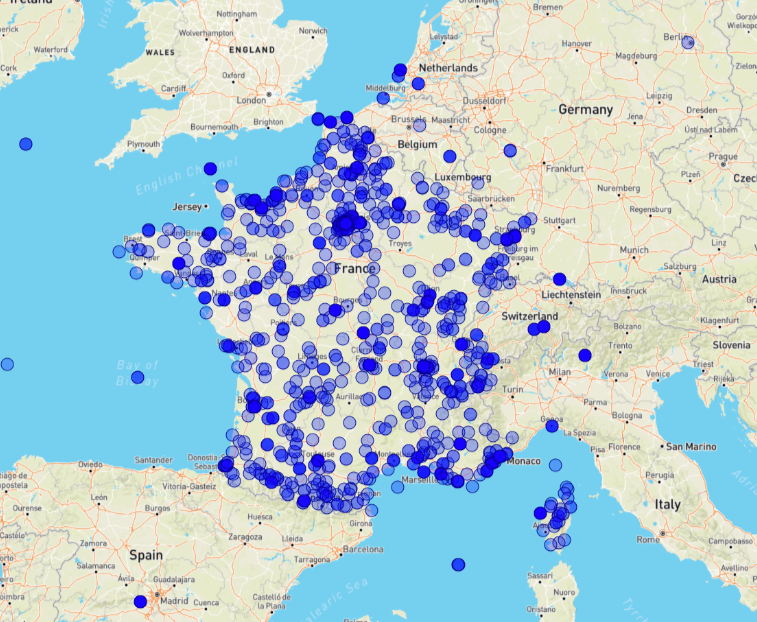
\includegraphics[width=0.9\textwidth]{imgs/france.png}
	\caption{First 1000 entities found that are connected to France. Entities are represented with a blue dot on the map.}
	\label{fig:france}
\end{figure}

The query is shown in Figure~\ref{fig:code_sparql}, which gives us $122,316$ entities found in the collection that have a connection with France (most of them are located in France). We can automatically show the entities on a map, as presented in Figure~\ref{fig:france} (showing the first 1000 entities found). 

Not all linked entities are located in France, however. For example, some entities are related to France (entities for which France is mentioned in their Wikidata) but located elsewhere in the world. One of the blue dots in Germany is the source of the river \emph{Moselle}. This river starts in Germany by splitting off from the \emph{Rhine}, and then goes through France. 
Instead of querying for France, we can also query for different countries. Table~\ref{tab:country_entities} shows the number of entities found for a sample of countries.

\begin{table}[]
	\caption{Number of entities found per country, for example countries where the entity has an English language label.}
	\label{tab:country_entities}
	\centering
	\begin{tabular}{l|c|r}
		\toprule
		Country & WikiData ID & \# Entities\\
		\midrule
		United States & Q30 & 3,429,889 \\
		Canada & Q16 & 170,833 \\
		France & Q146 & 122,316 \\
		New Zealand & Q664 & 19,094\\
		Peru & Q419 & 16,448 \\
		Iran & Q794 & 13,633\\
		Ecuador & Q736 & 10,588 \\
		South Korea & Q884 & 9,718\\
		Monaco & Q235 & 8,546\\
		Singapore & Q334 & 6,597\\
		\bottomrule
	\end{tabular}
\end{table}

\begin{figure}
	\centering
	\begin{minted}[linenos]{cypher}
MATCH (pid:Passage)-[:has]->(entity)
WHERE entity.uri CONTAINS "wikidata"
MATCH (pid)-[:description]->(content)
MATCH (entity)-[:label {lang: 'en'}]->(label)
MATCH (entity)-[:P625]->(coord)
MATCH (entity)-[:P17]->(:Country)
RETURN pid, content, entity, label, coord
	\end{minted}
	\caption{Cypher query with similar behaviour as the SPARQL query shown in~\ref{fig:code_sparql}.}
	\label{fig:code_geese}
\end{figure}

Although we have used SPARQL for this experiment, it would also be possible to express this query Cypher in GeeseDB. Depending on exact the schema, this would look like the query shown in~\cref{fig:code_geese}.

\section{Conclusion and Future Work}
This chapter introduces a new Information Retrieval resource called MMEAD, or MS MARCO Entity Annotations and Disambiguations. MMEAD contains entity annotations for the passages and documents in MS MARCO v1 and v2. These annotations simplify entity-oriented research on the MS MARCO collections. Links have been provided using the REL and BLINK entity linking systems. Using DuckDB, the data can quickly be queried, making the resource easy to use.
 
To return to our third research question:
\begin{itemize}
	\item[\textbf{RQ3:}] When does information retrieval research benefit from graph data?
\end{itemize}   

With MMEAD, we support information retrieval research that combines deep learning and entity graph information. Entity links can be considered a bi-partite graph where entities and documents are nodes, that are connected when entities appear in documents. Using these entities for query and passage expansion, we showed experimentally a significant increase in recall effectiveness. When using reciprocal rank fusion, the effectiveness difference becomes even more prominent and recall increases significantly with the new relevant passages found. The question remains open whether these passages previously missed, can be ranked higher by new retrieval models.

We also demonstrated that our resource can enrich interactive search applications. In particular, we present an demo where all entities related to geographical locations can be positioned on a map. Specifically we queried the data as a RDF triple graph.

Using the MMEAD format, releasing entity links for collections beyond MS MARCO is also possible. We already showed that using entity links improves recall when using the linked entities for query expansion. What the effects are when training, e.g., DPR methods that include the entity links, is yet to be investigated -- an exciting research opportunity that lies ahead. 

% \chapter{Data Modeling using Graphs}
\chapter{Conclusion}

\cleardoublepage
\phantomsection
\addcontentsline{toc}{chapter}{Bibliography}
\bibliographystyle{abbrvnat}
{
	\scriptsize
	\bibliography{./refs.bib}
}

\backmatter
% bibliography, glossary and index would go here.
\chapter*{Summary}
\addcontentsline{toc}{chapter}{Summary}
\markboth{Summary}{Summary}
\chapter*{Samenvatting}
\addcontentsline{toc}{chapter}{Samenvatting}
\markboth{Samenvatting}{Samenvatting}

Het vinden van relevante informatie in een grote verzameling van documenten is een zeer uitdagende taak, zeker wanneer alleen tekst in overweging wordt genomen bij het bepalen of een document relevant is. Dit onderzoek maakt gebruik van grafen om informatiebehoeften uit te drukken waar meer in overweging genomen moet worden dan alleen tekst. In sommige gevallen gebruiken we, voor de data representatie, in plaats van \emph{inverted indexes}, data management systemen om data op te slaan.

Allereerst, laten we zien dat relationele database systemen geschikt zijn voor \emph{information retrieval} experimenten.
Een door ons gebouwd prototype systeem implementeert een hele reeks verbeteringen aan het BM25-rangschikking algoritme die zijn voorgesteld in de literatuur. In een grootschalig reproductie onderzoek vergelijken we deze verbeteringen en vinden we dat de verschillen in effectiviteit kleiner zijn dan we op grond van de literatuur zouden verwachten. 
We kunnen gemakkelijk wisselen tussen versies van BM25 door de SQL-query slechts weinig te herschrijven met simpele variaties op een onderliggende SQL query. 

Hiermee valideren we het nut van relationele databases voor reproduceerbaar IR-onderzoek.
Vervolgens breiden we het datamodel uit naar een graaf datamodel. Met dit graaf datamodel kunnen we meer diverse gegevens uitdrukken dan alleen tekst. 
We kunnen complexe informatiebehoeften makkelijker uitdrukken met een bijbehorende graaf querytaal, dan wanneer een relationele taal wordt gebruikt. Dit model is gebouwd bovenop een \emph{embedded} database systeem, hierdoor kunnen we data dat geproduceerd wordt door dit systeem snel voor een andere applicatie gebruiken.

Een van de aspecten die we in de graaf vastleggen, is informatie over entiteiten. We gebruiken het Radboud Entity Linking (REL) systeem om entiteit informatie te koppelen aan documenten. Om een grote documentverzameling efficiënt te annoteren met REL hebben we de efficiëntie van REL verbeterd. Na deze verbeteringen hebben we REL gebruikt om annotaties te maken voor de MS MARCO-document- en passage-collecties. Met behulp van deze annotaties kunnen we de \emph{recall} voor moeilijkere MS MARCO-query's aanzienlijk verbeteren. Deze entiteiten worden ook gebruikt voor een interactieve demonstratie waarbij de geografische gegevens van entiteiten worden gebruikt.

\chapter*{Acknowlegements}
\addcontentsline{toc}{chapter}{Acknowlegements}
\markboth{Acknowlegements}{Acknowlegements}
\chapter*{Research Data Management}
\addcontentsline{toc}{chapter}{Research Data Management}
\markboth{Research Data Management}{Research Data Management}
\label{chp:research_data_management}

This thesis research has been carried out under the research data management policy of the Institute for Computing and Information Science of the Radboud University, the Netherlands\footnote{\url{https://www.ru.nl/icis/research-data-management/}}.

The following research datasets have been produced during this PhD research:

\begin{itemize}
	\item Resources for~\cref{ir-using-relational-databases}
	\begin{itemize}
		\item Code for OldDog~\citep{olddog-docker}:
		
		\href{https://doi.org/10.5281/zenodo.7892260}{chriskamphuis/olddog}: (v1.0.0). Zenodo. 10.5281/zenodo.3255060
		
		\item Code for the OldDog docker~\citep{olddog-docker}:
		
		\href{https://doi.org/10.5281/zenodo.3255060}{osirrc/olddog-docker}: (v1.0.0). Zenodo. 10.5281/zenodo.3255060
	\end{itemize}
	
	\item Resources for~\cref{from-tables-to-graphs}
	\begin{itemize}
		\item Code for GeeseDB~\citep{geesedb}:
		
		\href{https://doi.org/10.5281/zenodo.7892326}{informagi/GeeseDB}: (v0.0.2). Zenodo. 10.5281/zenodo.7892326
	\end{itemize}
	
	\item Resources for~\cref{a-graph-of-entities}
	\begin{itemize}
		\item Code for REBL~\citep{rebl}:
		
		\href{https://doi.org/10.5281/zenodo.7892359}{informagi/REBL}: (v0.0.1). Zenodo. 10.5281/zenodo.7892359
	\end{itemize}
	
	\item Resources for~\cref{mmead}
	\begin{itemize}
		\item Code for MMEAD~\citep{mmead}:
		
		\href{https://doi.org/10.5281/zenodo.7897027}{informagi/mmead}: (v0.1.0). Zenodo. 10.5281/zenodo.7897027
		
		\item Data for MMEAD~\citep{mmead}:
		
		\href{https://doi.org/10.5281/zenodo.7896782}{informagi/mmead}: (v0.0.1). Zenodo. 10.5281/zenodo.7896782
	\end{itemize}
	
\end{itemize}
\chapter*{Curriculum Vit\ae}
\addcontentsline{toc}{chapter}{Curriculum Vit\ae}
\markboth{Curriculum Vit\ae}{Curriculum Vit\ae}

\end{document}